\documentclass[10pt, a4paper, italian]{article}
\usepackage[T1]{fontenc}
\usepackage[utf8]{inputenc}
\usepackage{amsmath, amssymb, amsthm, thmtools, amsfonts, mathtools}
\usepackage{nicefrac}
\usepackage{calc}
\usepackage[pdftex, hyperindex, plainpages=false]{hyperref}
\usepackage[nameinlink]{cleveref} %load before classicthesis (clash)
%\usepackage[nochapters,pdfspacing]{classicthesis}
\usepackage{siunitx}
\usepackage[siunitx]{circuitikz}

\usepackage[a4paper]{geometry}
\usepackage{float}
\usepackage{mdframed}
\usepackage{titling}
\usepackage{booktabs}
\usepackage{graphicx}
\usepackage{caption, subcaption}
\usepackage{xcolor}
\usepackage[italian]{babel}
\usepackage{pgfplots}
\usepackage{listings}
%\usepackage{lmodern}
\usepackage{url}
\usepackage{enumitem}
\usepackage{tikz} %loads after classicthesis (xcolor incompat)

% lets graphicx know path where figures to be included are found
\graphicspath{{../figs/}}
\makeatletter
\def\input@path{{../figs/}}
%or: \def\input@path{{/path/to/folder/}{/path/to/other/folder/}}
\makeatother

% tikz pgf plots setup
\usepgfplotslibrary{external}
\pgfplotsset{compat=1.15}
%\tikzexternalize

% spaces and significant digits/figures for measurements
\sisetup{free-standing-units, space-before-unit, number-unit-product = \;,
scientific-notation = false, round-mode = figures, round-precision = 1,}

% turns all (hyperlinked) references black [default is blue]
\hypersetup{
	linktoc=all,
	colorlinks=true,
	linkcolor=black
}

% code listings config
%\lstset{
%language=Python,
%basicstyle=\ttfamily,
%columns=fullflexible,
%keepspaces=true,
%}

% mdframed (for boxed text) configuration
\mdfsetup{linewidth=0.6pt}

% Default fixed font does not support bold face
\DeclareFixedFont{\ttb}{T1}{txtt}{bx}{n}{12} % for bold
\DeclareFixedFont{\ttm}{T1}{txtt}{m}{n}{12}  % for normal

% Custom colors
\usepackage{color}
\definecolor{deepblue}{rgb}{0,0,0.5}
\definecolor{deepred}{rgb}{0.6,0,0}
\definecolor{deepgreen}{rgb}{0,0.5,0}

% Commands 
\newcommand{\executeiffilenewer}[3]{%
	\ifnum\pdfstrcmp{\pdffilemoddate{#1}}%
		{\pdffilemoddate{#2}}>0%
	{\immediate\write18{#3}}\fi%
}
% input .svg --> .pdf_tex graphs
%\newcommand{\includesvg}[1]{%
%	\executeiffilenewer{#1.svg}{#1.pdf}%
%	{inkscape -z -D --file=#1.svg %
%	--export-pdf=#1.pdf --export-latex}%
%	\input{#1.pdf_tex}%
%}
% Thanks UniPi's Department of Physics E. Fermi
\newcommand{\thanksdf}{(\thanks{Dipartimento di Fisica E.~Fermi,%
Universit\`a di Pisa - Pisa, Italy.}\;)}

% hyperlink to email address
\newcommand{\mail}[1]{\href{mailto:#1}{\textsf{#1}}}

% \vec for bold vectors, instead of overarrows (now "\arrvec")
\let\arrvec=\vec
\renewcommand{\vec}[1]{\boldsymbol #1}
% replaces straight phi with slanted phi
\renewcommand{\phi}{\varphi}
% replaces straight eps with curved epsilon
\newcommand{\eps}{\varepsilon}
% abbreviation for (sub_/super^)scripts of \lim, \sum,... in inline math
\newcommand{\ds}{\displaystyle}

% blackboard/number set letters
\newcommand{\CC}{\mathbb C}
\newcommand{\HH}{\mathbb H}
\newcommand{\KK}{\mathbb K}
\newcommand{\NN}{\mathbb N}
\newcommand{\PP}{\mathbb P}
\newcommand{\QQ}{\mathbb Q}
\newcommand{\RR}{\mathbb R}
\newcommand{\ZZ}{\mathbb Z}

\newcommand{\Abs}[1]{{\left\Vert #1\right\Vert}}
\newcommand{\enclose}[1]{{\left( #1 \right)}}
\newcommand{\Enclose}[1]{{\left[ #1 \right]}}
\newcommand{\floor}[1]{\left\lfloor #1 \right\rfloor}
\newcommand{\ceil}[1]{\left\lceil #1 \right\rceil}
\newcommand{\To}{\rightrightarrows}

% Math operators
\DeclareMathOperator{\divergence}{div}
\renewcommand{\div}{\divergence}
\DeclareMathOperator{\Imaginarypart}{Im}
\renewcommand{\Im}{\Imaginarypart}
\DeclareMathOperator{\Realpart}{Re}
\renewcommand{\Re}{\Realpart}
%\DeclareMathOperator{\arg}{arg}
\DeclareMathOperator{\tg}{tg}
\DeclareMathOperator{\arctg}{arctg}
\DeclareMathOperator{\settsinh}{settsinh}
\DeclareMathOperator{\settcosh}{settcosh}
\DeclareMathOperator{\tr}{tr}
\DeclareMathOperator{\im}{im}
\DeclareMathOperator{\sgn}{sgn}
\DeclareMathOperator{\diag}{diag}

\DeclarePairedDelimiter{\norm}{\lVert}{\rVert}
\DeclarePairedDelimiter{\scalar}{\langle}{\rangle}

% Logarithm with arbitrary base.
% -> log_10
\newcommand{\llog}[1][10]{\log_{#1}}

% Absolute value.
% -> |x|
\newcommand{\abs}[1]{\left| #1 \right|}

% Powers.
% -> x^a
\newcommand{\power}[2][2]{\left( #2 \right)^{#1}}

% Square.
% -> x^2
\newcommand{\sq}[1]{\power[2]{#1}}

% Expansion of the binomial coefficient.
% -> n1!/(n2!(n1 - n2)!)
\newcommand{\binomexpr}[2]{\frac{#1!}{#2!(#1 - #2)!}}

% Expression evaluation at a given point with square brackets.
% -> [x]_{a}
\newcommand{\at}[2]{\left[ #1\right]_{\makebox[-1pt][l]{${\scriptstyle#2}$}}}

% Expression evaluation in an interval.
% -> [x] _{a}^{b}
\newcommand{\eval}[3]{\left.#1%
  \right|_{\makebox[-1pt][l]{${\scriptstyle#2}$}}^{\makebox[-1pt][l]{${\scriptstyle#3}$}}}

% Upright d in math mode (for differentials).
% -> d
\newcommand{\ud}{\mathrm{d}}

% Differential.
% -> dx
\newcommand{\diff}[1][x]{\,\ud{#1}}

% Base command for defining derivatives.
% -> df/dx or d^kf/dx^k
\newcommand{\basederivative}[4][]{%
  \displaystyle%
  \ifx\\#1\\\frac{#4#2}{#4#3}%
  \else%
  \frac{#4^#1#2}{#4#3^#1}%
  \fi%
}

% Total derivative.
% -> df/dx(x) or d^kf/dx^k(x)
\newcommand{\td}[4][]{%
  \basederivative[#1]{#2}{#3}{\ud}%
  \ifx\\#4\\%
  \else%
  \mkern-4mu\left(#4\right)%
  \fi%
}

% Partial derivative.
% -> df/dx(x) or d^kf/dx^k(x)
\newcommand{\pd}[4][]{%
  \basederivative[#1]{#2}{#3}{\partial}%
  \ifx\\#4\\%
  \else%
  \mkern-4mu\left(#4\right)%
  \fi%
}

\newcommand{\intinf}{\int_{-\infty}^{\infty}\!\!\!}

\newcommand{\cinterval}[2]{\left[\, #1,~#2 \,\right]}

\newcommand{\linterval}[2]{\left[\, #1,~#2 \,\right)}

\newcommand{\rinterval}[2]{\left(\, #1,~#2 \,\right]}

\newcommand{\ointerval}[2]{\left(\, #1,~#2 \,\right)}

\newcommand{\prob}[1]{\displaystyle P\left(#1\right)}

\newcommand{\pvalue}{\emph{$p$-value}}

\newcommand{\cond}{\,|\,}

\newcommand{\expect}[1]{\displaystyle E\left[#1\right]}

\newcommand{\mom}[2][]{\displaystyle {\cal M}_{#2}\ifx\\#1\\\else(#1)\fi}

\newcommand{\momalg}[1]{\displaystyle \lambda_{#1}}

\newcommand{\momcen}[1]{\displaystyle \mu_{#1}}

\newcommand{\skewness}{\displaystyle \gamma_1}

\newcommand{\kurtosis}{\displaystyle \gamma_2}

\newcommand{\charf}[1][x]{\phi_{#1}}

\newcommand{\momgenf}[1][x]{M_{#1}}

\newcommand{\fwhm}{{\scriptstyle \textsc{FWHM}}}

\newcommand{\hwhm}{{\scriptstyle \textsc{HWHM}}}

\newcommand{\median}{\mu_{\nicefrac{1}{2}}}

\newcommand{\var}[1]{\ensuremath{\text{Var}\left(#1\right)}}

\newcommand{\cov}[2]{\ensuremath{\text{Cov}\left(#1, #2\right)}}

\newcommand{\corr}[2]{\ensuremath{\text{Corr}\left(#1, #2\right)}}

\newcommand{\like}{\mathcal L}

\newcommand{\likelihood}[2][]{\like\ifx\\#2\\\else(#2\ifx\\#1\\\else;#1\fi)\fi}

\newcommand{\chisq}{\ensuremath{\chi^2}}

\newcommand{\chisquare}[2][]{\chisq\ifx\\#2\\\else(#2\ifx\\#1\\\else;#1\fi)\fi}

\newcommand{\loglikelihood}[2][]{\log\likelihood[#1]{#2}}

\newcommand{\pdf}[3][]{#2(#3\ifx\\#1\\\else;#1\fi)}

\newcommand{\binomialpdf}[2][]{\pdf[#1]{\mathcal B}{#2}}

\newcommand{\multinomialpdf}[2][]{\pdf[#1]{\mathcal M}{#2}}

\newcommand{\poissonpdf}[2][]{\pdf[#1]{\mathcal P}{#2}}

\newcommand{\uniformpdf}[2][]{\pdf[#1]{u}{#2}}

\newcommand{\exponentialpdf}[2][]{\pdf[#1]{\varepsilon}{#2}}

\newcommand{\gausspdf}[2][]{\pdf[#1]{N}{#2}}

\newcommand{\chisquarepdf}[2][]{\pdf[#1]{\wp}{#2}}

\newcommand{\cauchypdf}[2][]{\pdf[#1]{c}{#2}}

\newcommand{\erf}[1]{\ensuremath{\text{erf}\left(#1\right)}}

\newcommand{\dccases}[4][]{#2 \ifx\\#2\\\else=\fi %
  \begin{cases}
    \displaystyle #3 & \text{per variabili discrete}\\
    \displaystyle #4 & \text{per variabili continue}#1
  \end{cases}
}
% sub/super-scriptable for all symbol as math operator 
\newcommand\Scaleforall[1]{\vcenter{\hbox{\scalefont{#1}$\forall$}}}

\DeclareMathOperator*\forevery{%
  \vphantom\sum
  \mathchoice{\Scaleforall{2}}{\Scaleforall{1.4}}{\Scaleforall{1}}{\Scaleforall{0.75}}}
\usepackage{multicol}
\usepackage{diagbox}
\geometry{left=2cm, right=2cm, top=2cm, bottom=2cm}

% indexes subsections with letters, sections with numbers (1.a, 1.b, ...)
\renewcommand{\thesubsection}{\thesection.\alph{subsection}}

% lets graphicx know path where figures to be included are found
\graphicspath{{../figs/}}

\author{Gruppo 1.AC \\ Matteo Rossi, Bernardo Tomelleri}
\title{EsD1: Caratterizzazione di porte logiche e semplici circuiti logici.}
\begin{document}
\date{\today}
\maketitle

\section*{Misura componenti dei circuiti}
\begin{table}[htbp]
\centering
\begin{tabular}{ccc}
\toprule
Resistenze $[\si{\ohm}]$ & $R$ & $\sigma R$ \\
\midrule
\midrule
$R\ped{pot1}$	& 9.53 k	& 0.08 k 		\\
$R\ped{pot2}$	& 9.78 k	& 0.08 k 		\\

\bottomrule     
\end{tabular}
\caption{Valori di resistenza misurati per i componenti passivi dei circuiti
studiati. \label{tab: rmesM}}
\end{table}

Riportiamo per completezza anche il valore della tensione continua di
alimentazione per i circuiti integrati misurata con il multimetro
\begin{align*}
V_{CC} &= 4.99 \pm 0.03 \si{\V} \\
\end{align*}

\subsection*{Nota sul metodo di fit}
Per determinare i parametri ottimali e le rispettive covarianze si \`e
implementato in \verb+Python+ un algoritmo di fit basato sui minimi quadrati
mediante la funzione \emph{curve\_fit} della libreria \texttt{SciPy}.

\setcounter{section}{0}
%=======================
\section*{Parte A: Caratteristiche fisiche delle porte logiche}
Si studia il comportamento delle porte NOT TTL contenute nel circuito integrato SN7404 misurando le tensioni e correnti di operazione e verificando che queste rientrino nelle specifiche tecniche riportate nel Data-Sheet del chip in \cref{fig: SN7404}.
\begin{minipage}{0.3\textwidth}
    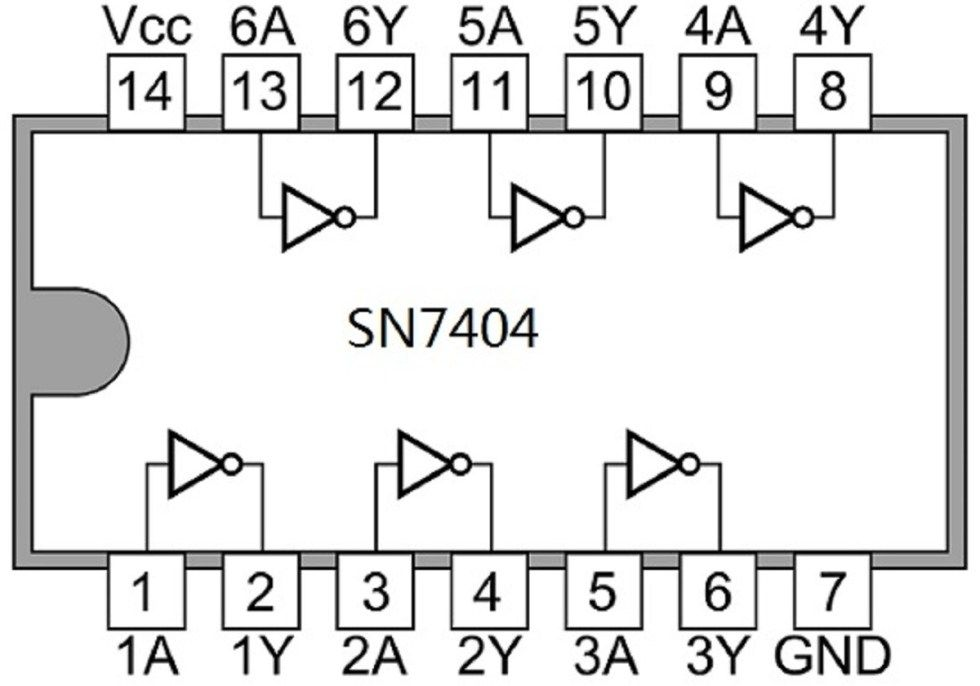
\includegraphics[width=\textwidth]{SN7404}
    
    \label{fig: SN7404}
\end{minipage}

\section{Tensioni di operazione}\label{sec: tens}
Per prima cosa misuriamo i valori delle tensioni di soglia in ingresso e in
uscita (e verifichiamo che rispettino le specifiche di buon funzionamento del
DS) da cui è possibile ottenere una misura del Noise Margin delle porte.

Dalle specifiche del DS si ha che i valori attesi sono: (riportati in
\cref{tab: notDS})
\begin{table}[htb]
\centering
\begin{tabular}{cccc|c}
\toprule
Parameter  & min & typ & max & [Unit] \\
\midrule
\midrule
$V_{CC}$ &  &  & $7$ & V \\
$V_I$	 &  &  & $5.5$ & V\\
$V_{OH}$ & $2.4$  & $3.4$ & & V \\
$V_{OL}$ &   & $0.2$ & $0.4$ & V \\
$V_{IH}$ & $2$  &  & & V  \\
$V_{IL}$ &  &  & $0.8$ & V \\
$I_{IH}$ &  &  & $40$ & $\si{\micro\A}$ \\
$I_{OH}$ &  &  & $-0.4$ & mA \\
\bottomrule 
\end{tabular}
\caption{Valori delle tensioni e correnti di operazione indicati sul
datasheet dell'integrato SN7404.}
\label{tab: notDS}
\end{table}

in cui $V_O$ e $V_I$ sono definite come le tensioni in uscita e in ingresso
dalla porta logica (le altre diciture indicano se la grandezza a cui facciamo
riferimento corrisponde a uno stato logico alto (H) o basso (L) e quali sono
i massimi o minimi valori garantiti dal costruttore).

\subsection{Misura delle tensioni di soglia dal grafico
$V\ped{out}(V\ped{in})$}
Generiamo una rampa di tensione compresa tra 0-5 V e la inviamo
all'ingresso di una porta NOT per osservare i segnali generati in uscita,
così da ottenere un grafico di $V\ped{out}$ in funzione di $V\ped{in}$.

Abbiamo quindi utilizzato i cursori per misurare $V_{OH}$ e $V_{OL}$, cioè
la tensione che raggiunge l'uscita in saturazione per valore logico H e L
rispettivamente, mentre per misurare $V_{IL}$ e $V_{IH}$ abbiamo misurato le
tensioni in ingresso per cui inizia e finisce la commutazione dell'uscita
secondo lo schema in \cref{fig: trans}:
\begin{figure}[htbp]
\centering
	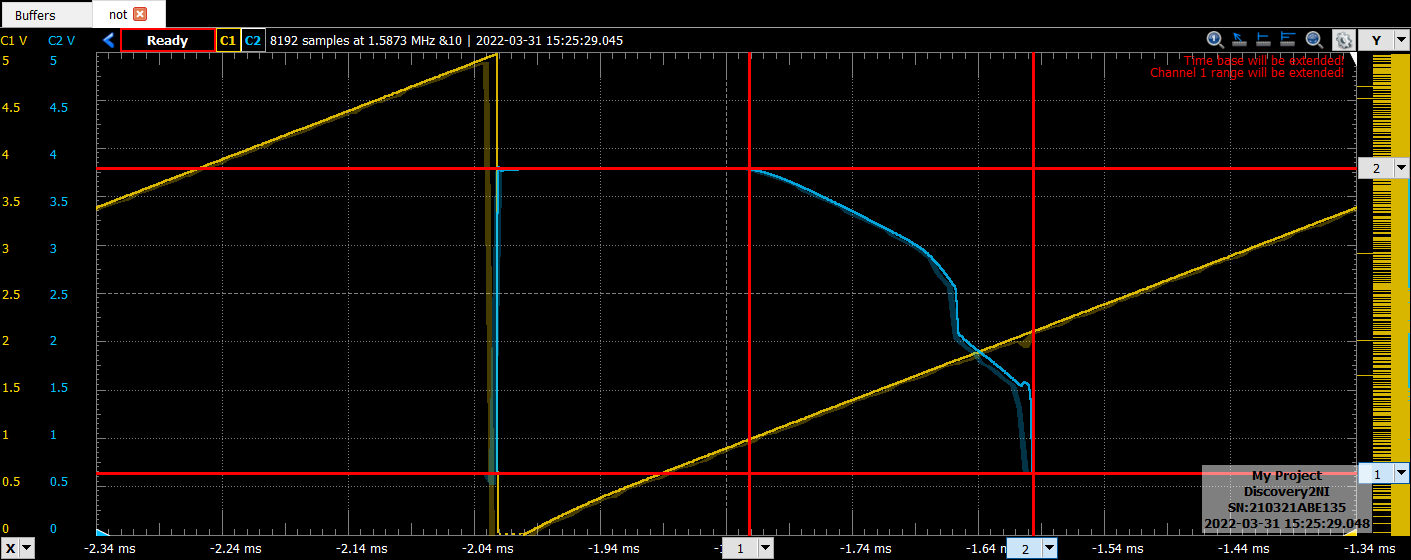
\includegraphics[width=\textwidth]{trans}
	\caption{Schema di come sono stati utilizzati i cursori per misurare le tensioni $V_{OH}$, $V_{OL}$ (cursori orizzontali) e $V_{IH}$, $V_{IL}$ (aiutandosi con i cursori verticali a individuare la fase di transizione H->L)}
	\label{fig: trans}
\end{figure}
\begin{multicols}{2}
    \centering
    $V_{OH} = 3.78 \pm 0.03\; \si{\V}$ \\
	$V_{OL} = 632 \pm 4 \; \si{m\V}$ \\
	$V_{IH} = 2.10 \pm 0.02 \; \si{\V} $\\
	$V_{IL} = 979 \pm 9\; \si{m\V} $\\
    
    $V_{OH} = 3.76 \pm 0.03\; \si{\V}$ \\
	$V_{OL} = 341 \pm 3 \; \si{m\V}$ \\
	$V_{IH} = 1.81 \pm 0.02 \; \si{\V} $\\
	$V_{IL} = 772 \pm 8\; \si{m\V} $\\
\end{multicols}

\begin{figure}[htbp]
\centering
	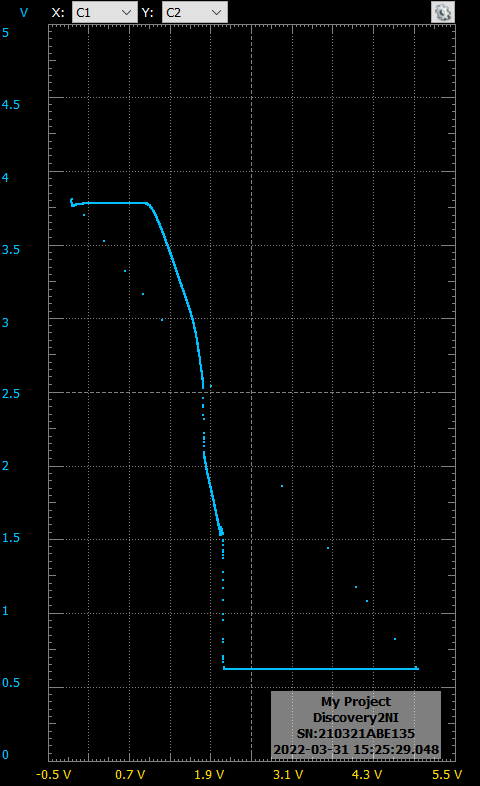
\includegraphics[scale=0.4]{not_xy1}
	\caption{Grafico XY di $V\ped{out}$ in funzione di $V\ped{in}$}
\end{figure}
\begin{figure}[htbp]
\centering
	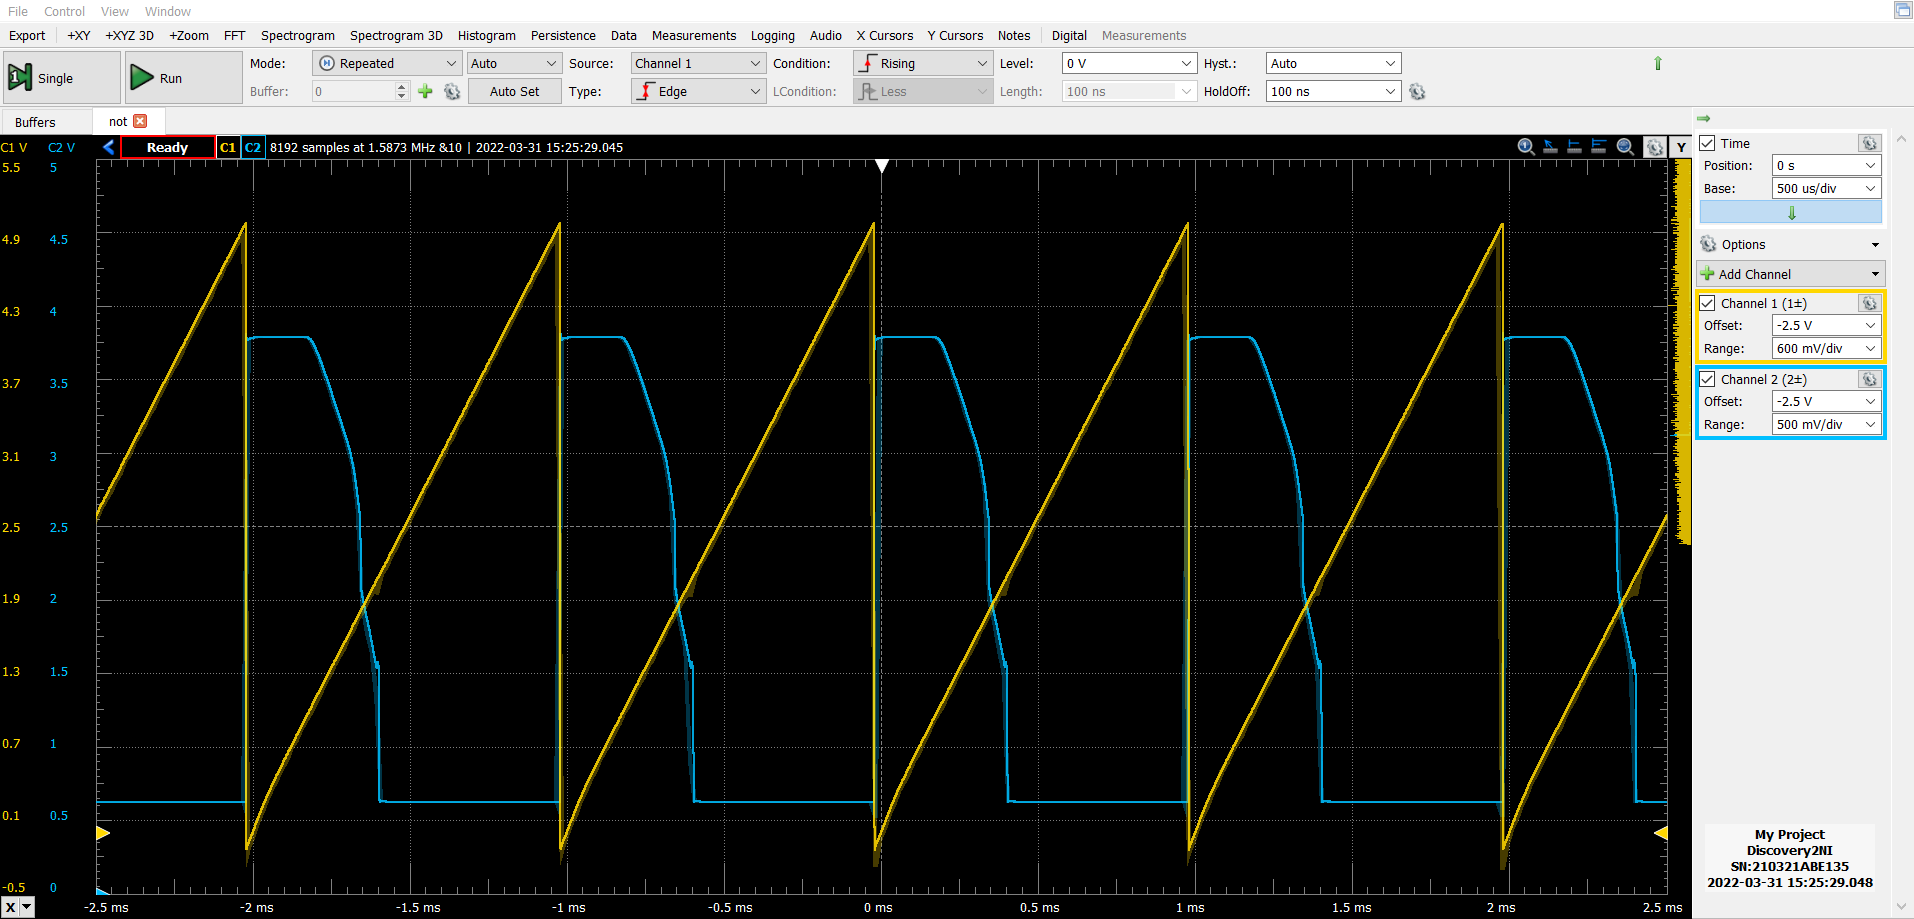
\includegraphics[width=\textwidth]{not_time1}
	\caption{Grafico in funzione del tempo di $V\ped{in}$ (in giallo, una rampa da 0 a 5 V di frequenza pari a 1 kHz) e $V_{out}$ (in blu)}
\end{figure}

Sempre con i cursori abbiamo misurato $V\ped{OH, min}$ dato che il valore
minimo per lo stato alto dell'uscita risultava più basso di
quanto misurato prima; di conseguenza abbiamo spostato il cursore nel punto
in cui la tensione in uscita cambia in maniera più repentina:
\begin{figure}
\centering
	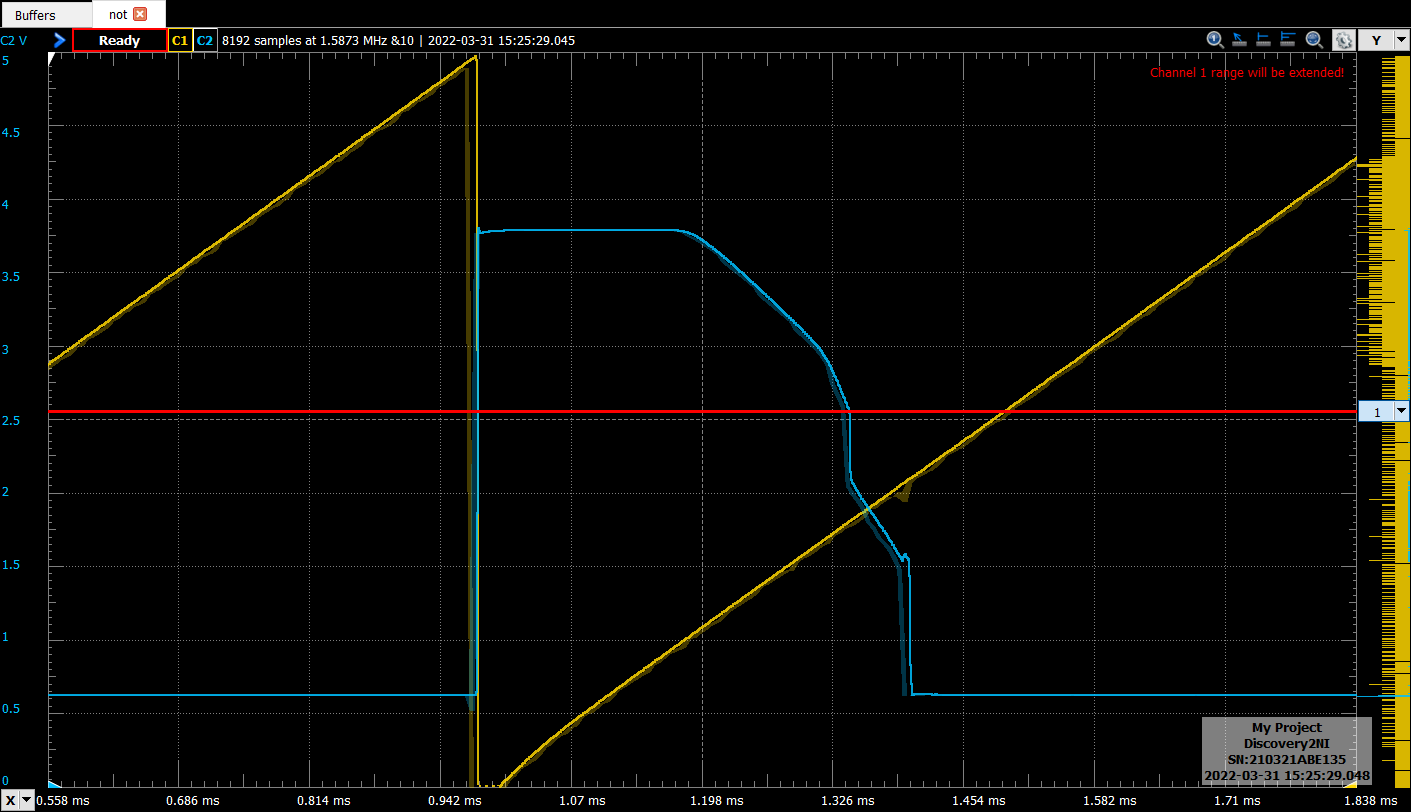
\includegraphics[scale=0.4]{trans1}
	\caption{Schema di come è stata presa la misura di $V\ped{OH, min}$ tramitel'utilizzo dei cursori: è stato scelto come valore minimo la tensione dell'uscita subito prima del primo cambio repentino.}
	\label{fig: trans1}
\end{figure}
Successivamente si sono utilizzati gli altri valori presi in precedenza per completare le misure.
Per il primo integrato:
\begin{multicols}{2}
    \centering
    $V\ped{OH, min}=$ 2.53 $\pm$ 0.03 V\\
    $V\ped{IH, min}=$ 2.10 $\pm$ 0.02 V\\
    
    $V\ped{IL, max}=$ 979 $\pm$ 9 mV\\
    $V\ped{OL, max}=$ 632 $\pm$ 4 mV\\
\end{multicols}
mentre per il secondo:
\begin{multicols}{2}
    \centering
    $V\ped{OH, min}=$ 2.40 $\pm$ 0.03 V\\
    $V\ped{IH, min}=$ 1.81 $\pm$ 0.02 V\\
%    $NM_H=$ 0.60 $\pm$ 0.04 V
    
    $V\ped{IL, max}=$ 772 $\pm$ 8 mV\\
    $V\ped{OL, max}=$ 341 $\pm$ 3 mV\\
%    $NM_L=$ 0.43 $\pm$0.01 V
\end{multicols}

Da cui troviamo le nostre stime dei valori delle soglie di rumore (Noise
Margin High e Low) per le porte NOT studiate, definite come
\begin{multicols}{2}
\begin{align*}
NM_H = V\ped{OH, min} - V\ped{IH, min} &= (0.43 \pm 0.04) \; \si{\V} \\
    &= (0.60 \pm 0.03) \; \si{\V}
\end{align*}

\begin{align*}    
NM_L = V\ped{IL, max} - V\ped{OL, max} &= (0.35 \pm 0.02) \; \si{\V} \\
    &= (0.43 \pm 0.02) \; \si{\V}
\end{align*}
\end{multicols}

\subsection{Valori attesi per le soglie di rumore}
Estrapolando i corrispettivi valori dal datasheet, e assumendo che ogni porta
logica abbia i medesimi parametri delle altre presenti nello stesso integrato
possiamo allora ricavare i valori attesi dei Noise Margin High e Low:
\begin{align*}
NM_H = 2.4 - 2 = 0.4 \; \si{\V} \\
NM_L = 0.8 - 0.4 = 0.4 \; \si{\V}
\end{align*}

\subsection{Confronto dei risultati}
Le nostre misure risultano compatibili con le aspettative entro gli intervalli
ammessi dal datasheet per il buon funzionamento del componente, dunque anche
le grandezze derivate risultano in accordo con le aspettative.

\section{Misura (statica) del Fan-out}
Chiamiamo Fan-Out il massimo numero di porte che una singola porta è in grado
di pilotare rimanendo entro le specifiche di funzionamento del datasheet, lo
si è definito come
\[
\text{FO}= \abs{\frac{I\ped{IH, max}}{I\ped{OH, max}}}
\]

\subsection{Misura della corrente in ingresso alla porta NOT nello stato alto}
Misuriamo la corrente $I\ped{IH, max}$ per entrambi gli integrati collegando
l'amperometro in serie tra l'ingresso della porta logica e l'uscita del
canale WaveGen1 dell'AD2, quindi generando in questo canale una tensione
continua di livello alto pari a 5 V, da cui si trova
\begin{align*}
    I\ped{IH, 1} &= 16 \pm 1 \; \si{\micro\A} \\
    I\ped{IH, 2} &= 10 \pm \; \si{\micro\A} \\   
\end{align*}
Che risultano essere compatibili entro i limiti del datasheet.

\subsection{Misura della corrente in uscita dalla porta NOT per VOH tipico}
Successivamente abbiamo inviato all'ingresso della porta un segale DC a 0 V
(sempre utilizzando il canale WG1) e abbiamo inserito un potenziometro da
$10 \; \si{k\ohm}$ in serie all'uscita di questa per misurare la corrente che
scorre attraverso questa ``resistenza di carico'' regolabile in modo da
avere quando una tensione in uscita dalla porta corrispondente al valore
tipico di $V_{OH}= 3.40 \pm 0.03 \; \si{\V}$.
\begin{align*}
    I\ped{OH, 1} &= 495 \pm 4 \; \si{\micro\A} \\
    I\ped{OH, 2} &= 315 \pm 3 \; \si{\micro\A} \\   
\end{align*}

\subsection{Misura della corrente in uscita dalla porta NOT per VOH tipico}
%TODO inseirire cosa sarebbe successo se avessi abbassato la tensione in
%uscita ai valori di VOH 2.5 V (min) o 3.8 V (saturazione) circa

\subsection{Misura indiretta del fan-out}
Dalle misure di corrente sui due integrati ricaviamo finalmente che:
\begin{align*}
    \text{FO}_1 &= 31 \pm 2 \\
    \text{FO}_2 &= 32 \pm 3 \\
\end{align*}

\subsection{Valore del fan-out atteso e confronto}
Dalle specifiche del DS elencate sopra in \ref{tab: notDS} risulta che
\begin{align*}
    I\ped{IH, max}= -0.4 \; \si{m\A} \\
    I\ped{OH, max}= 40 \; \si{\micro\A} \\
    \text{FO} = 10
\end{align*}
I valori da noi trovati risultano sensibilmente più alti delle aspettative
e non compatibili con queste, ma perlomeno rimangono compatibili tra di loro.

\section{Tempi di propagazione}
Vogliamo ora misurare i tempi di propagazione della porta logica NOT
osservando (tramite un oscilloscopio da banco) l'andamento nel tempo dei
segnali nei pin di ingresso uscita della porta durante le transizioni di stato
per poi paragonarli ai valori riportati sul datatsheet in analogia a quanto
fatto finora.

\subsection{Definizione e valori attesi dei tempi di propagazione}
Dal datasheet TI fornito le misure di tempi di propagazione per la commutazione
dell'uscita tra gli stati alto->basso $t_{PHL}$ e basso->alto $t_{PLH}$ sono
definite come l'intervallo di tempo tra il passaggio della forma d'onda in
ingresso e di quella in uscita dal livello di tensione iniziale al punto
medio tra lo stato iniziale e finale, secondo lo schema in 

\begin{figure}[htbp]
\centering
	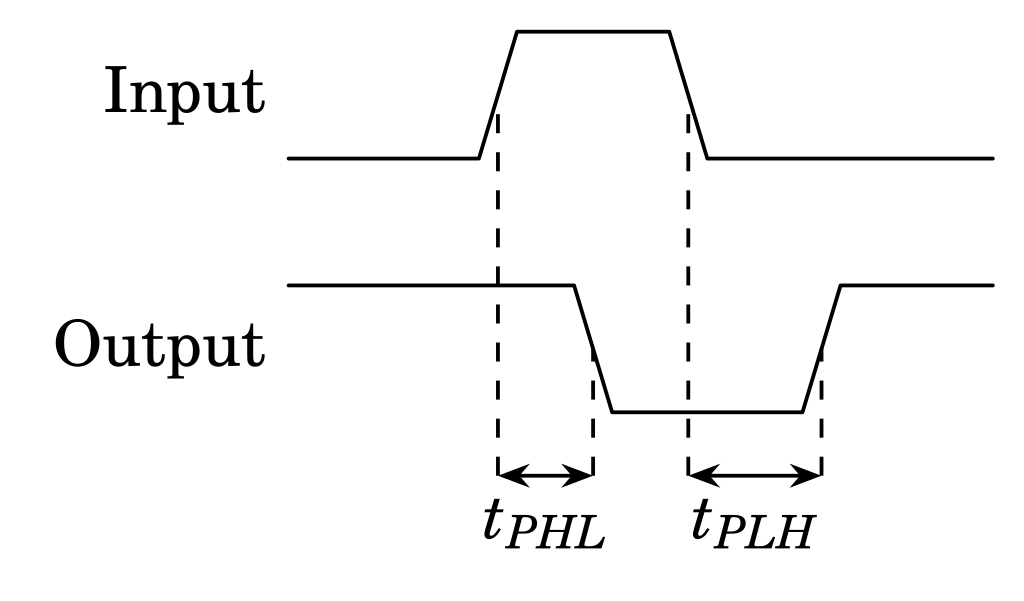
\includegraphics[scale=0.4]{notdelay}
	\caption{Diagramma dei tempi di propagazione per una porta NOT}
\end{figure}

Prendiamo quindi come definizione di tempo di propagazione il lasso di tempo
che trascorre tra quando $V\ped{in}$ diventa pari a $V\ped{I, med}$ e
$V\ped{out}$ diventa pari al suo $V\ped{O, med}$, dove i valori medi tra stato
basso e stato alto rispettivamente per l'ingresso e per l'uscita sono
definiti intuitivamente dalle formule
\begin{align*}
V\ped{O, med} &= \frac{V_{OH} + V_{OL}}{2} \\
V\ped{I, med} &= \frac{V_{IH} + V_{IL}}{2} \\
\end{align*}

Dal datasheet si ricavano come tempi di propagazione attesi:
\begin{align*}
    t_{PHL,max} &= 22 \; \si{n\s} \\
    t_{PLH,max} &= 15 \; \si{n\s} \\
\end{align*}

\subsection{Misura dei tempi con l'oscillografo}
Come visto anche nella \cref{sec: tens}, inviando in ingresso un'onda quadra
compresa tra 0 e 5 V, all'uscita della porta troviamo la stessa onda compresa
tra $V_{OH} \approx 3.6 \; \si{\V}$ e $V_{OL} \approx 0.3  \; \si{V}$;
infatti misurando con i cursori e con l'oscilloscopio troviamo come
\begin{align*}
V\ped{O, med} = 1.95 \pm 0.02 \\
V\ped{I, med} = 2.50 \pm 0.03 \\
\end{align*}

Quindi, una volta collegati i due canali all'ingresso (CH1) e all'uscita (CH2)
del not gate, abbiamo scelto come evento di trigger il passaggio del segnale
di ingresso per $V_{I,med}$, abbiamo dunque cambiato il fronte tra
salita/discesa per scegliere se misurare il tempo di propagazione H->L o L->H.
\begin{figure}[htbp]
\centering
	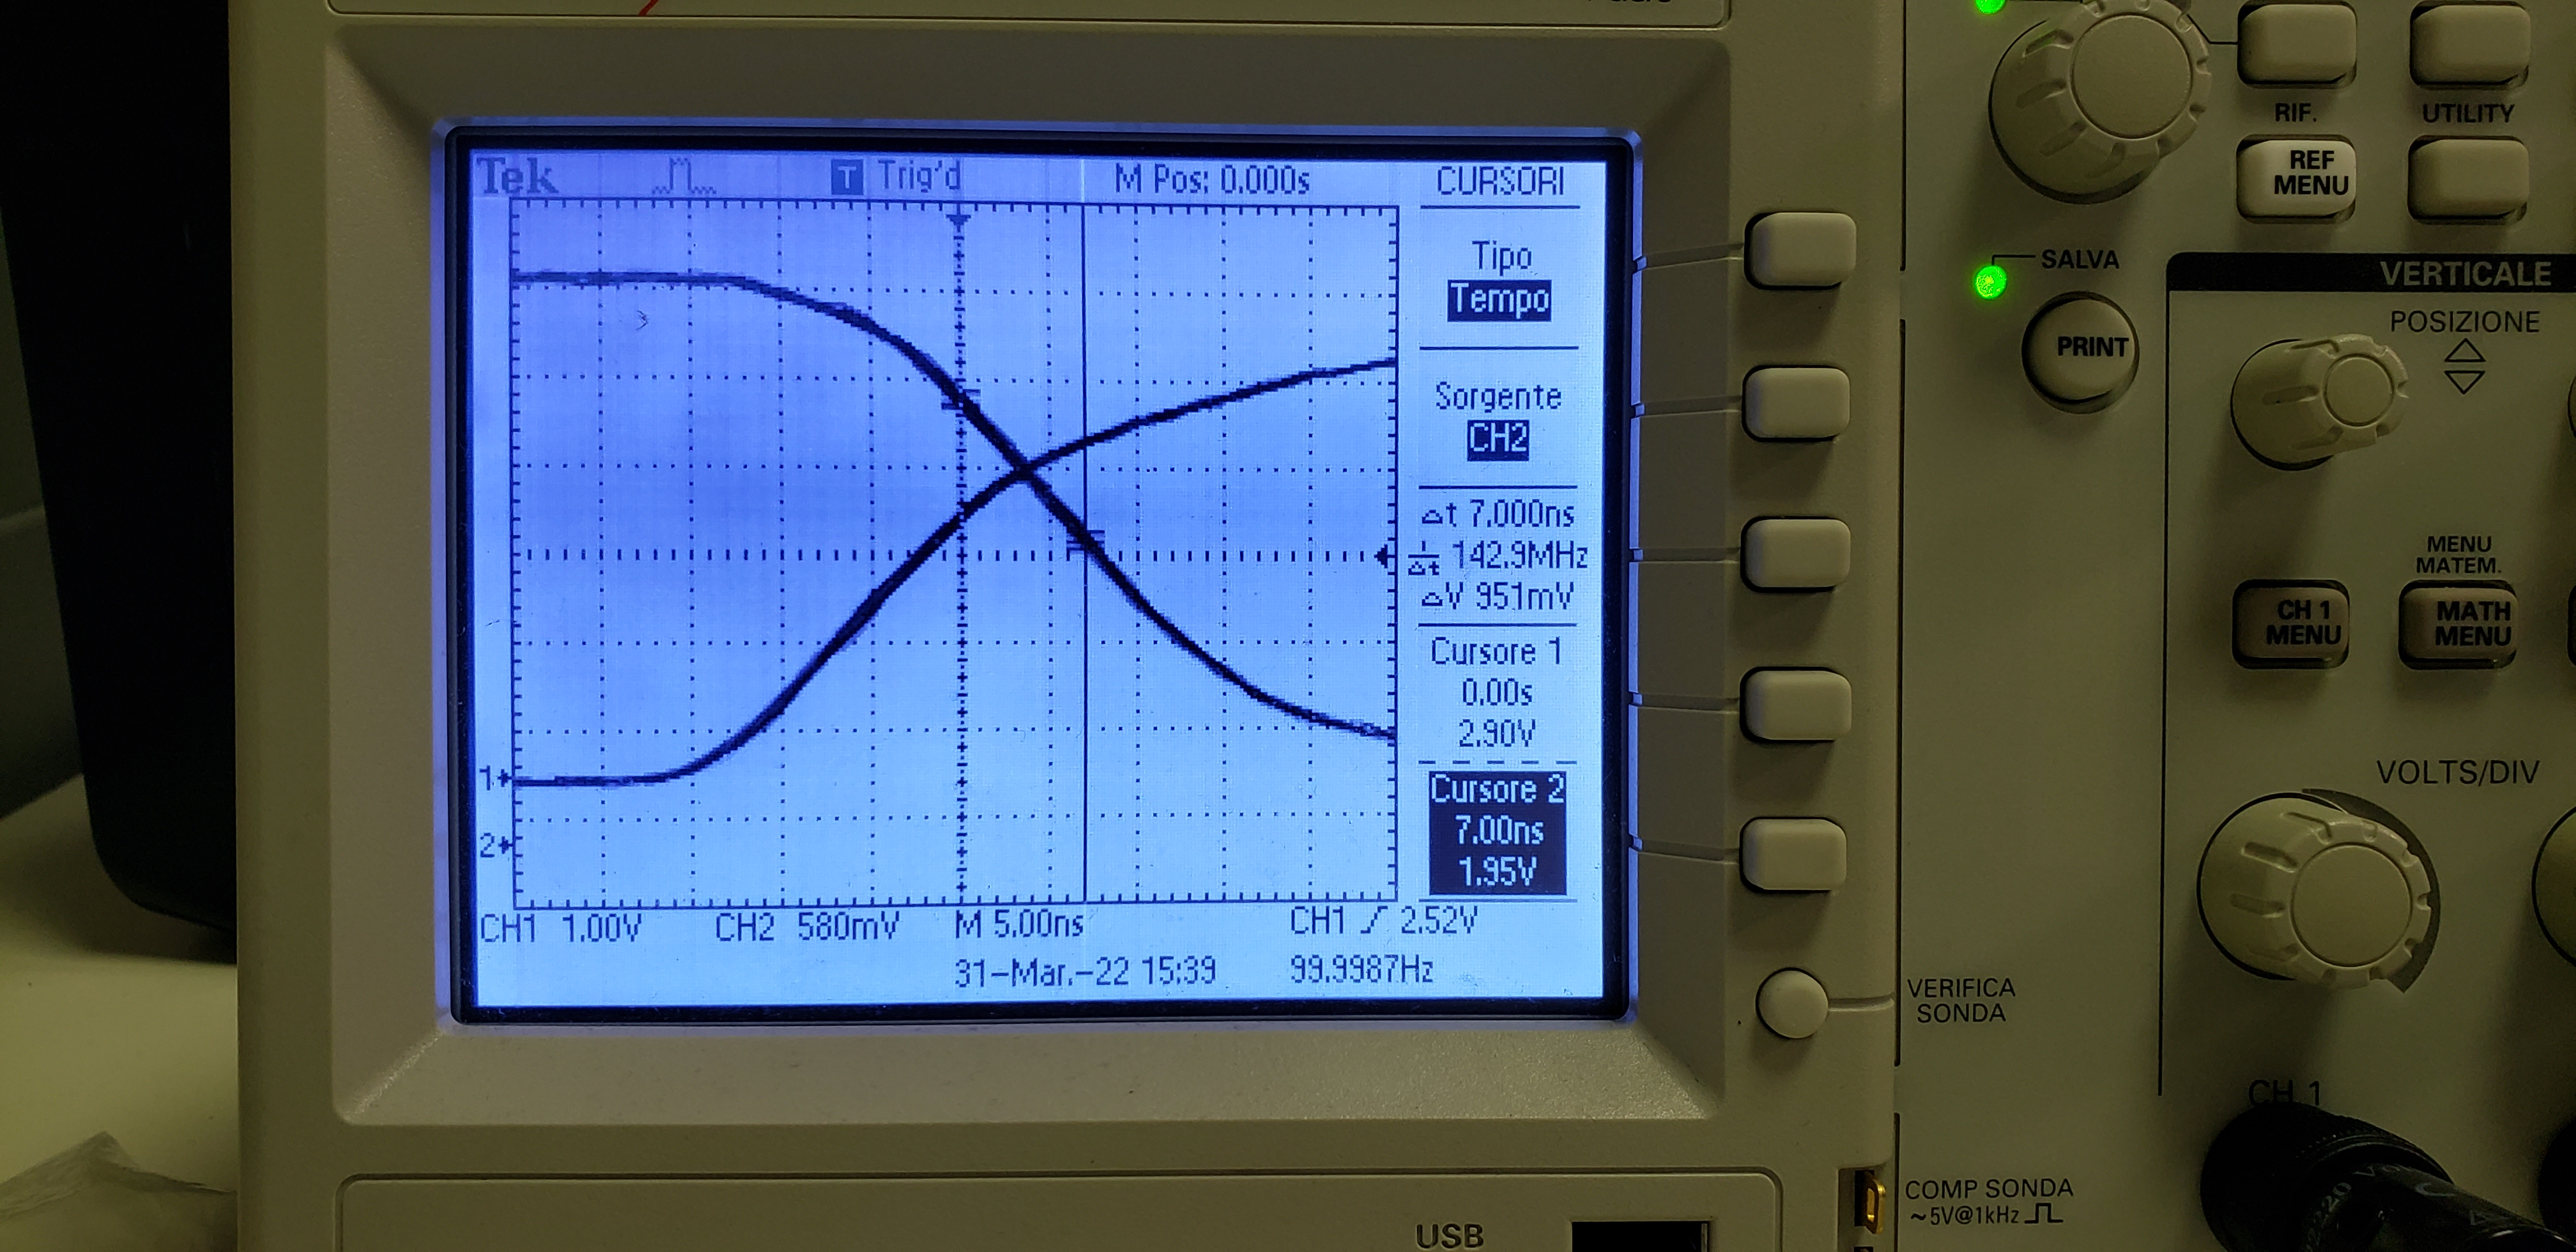
\includegraphics[width=\textwidth]{LH1}
	\caption{Acquisizione tramite oscilloscopio digitale della transizione da
	L a H per il primo integrato}
\end{figure}
\begin{figure}[htbp]
\centering
	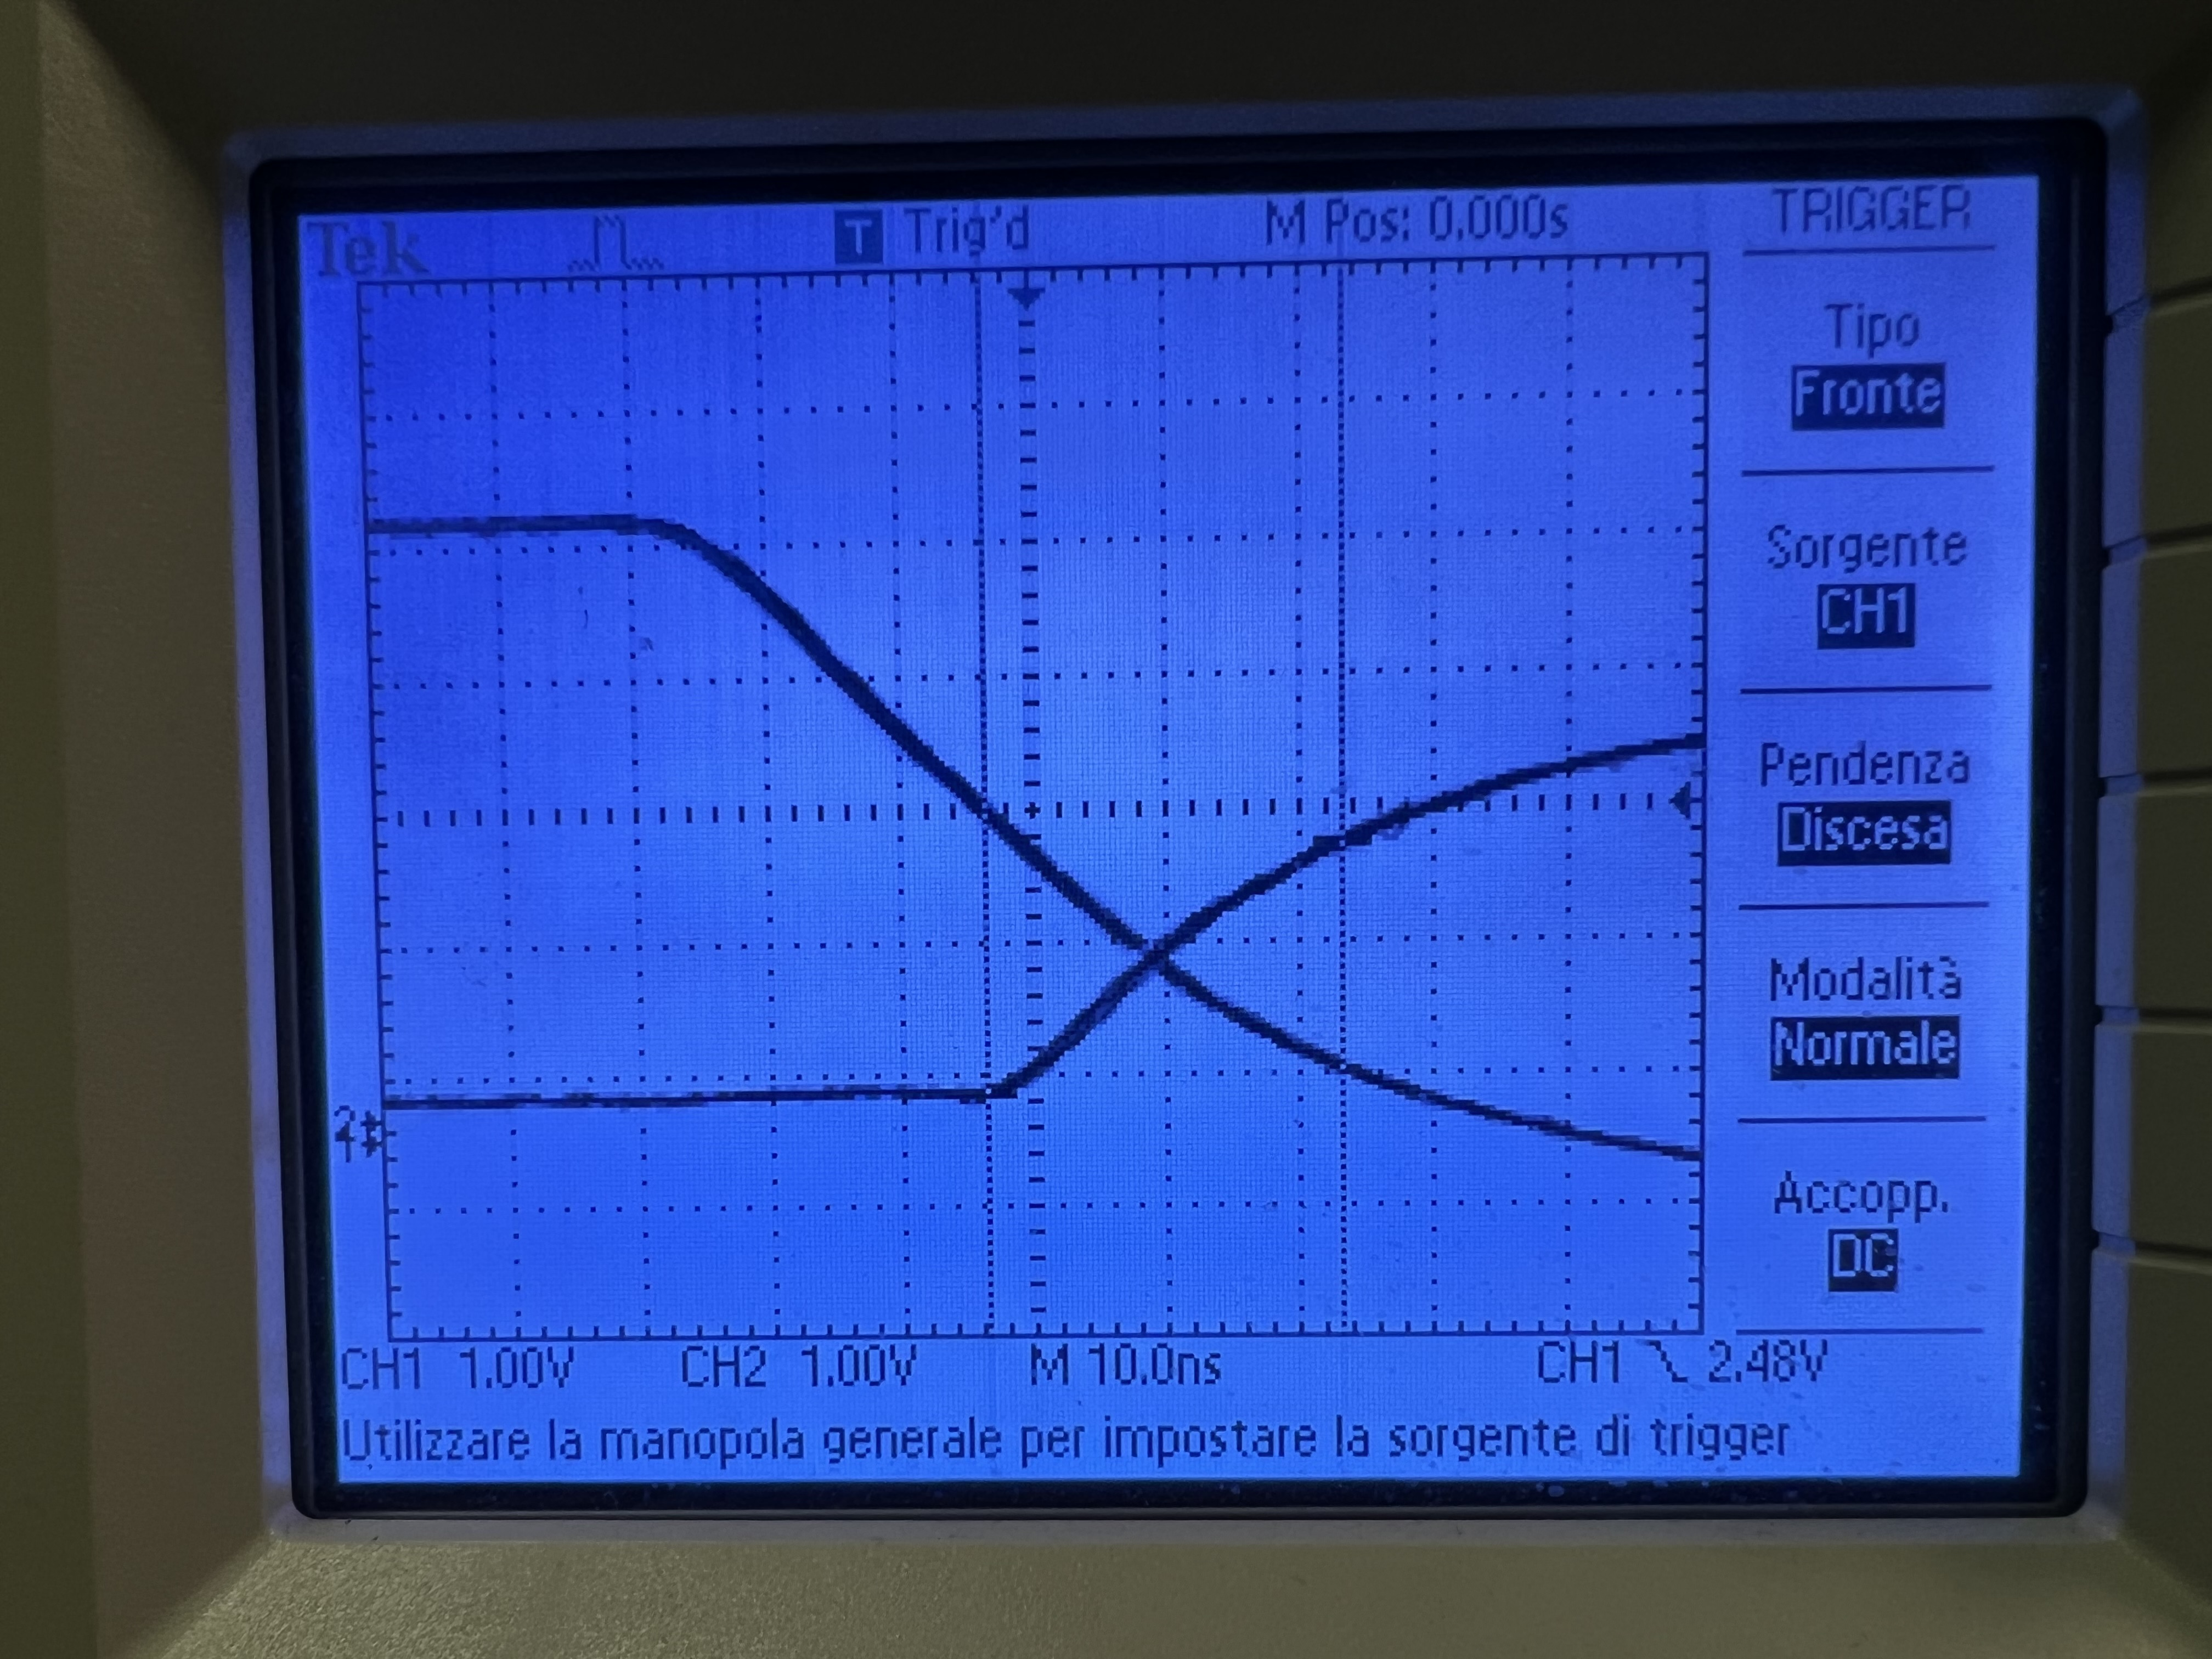
\includegraphics[width=\textwidth]{LH2}
	\caption{Acquisizione tramite oscilloscopio digitale della transizione da
	L a H per il secondo integrato}
\end{figure}
\begin{figure}[htbp]
\centering
	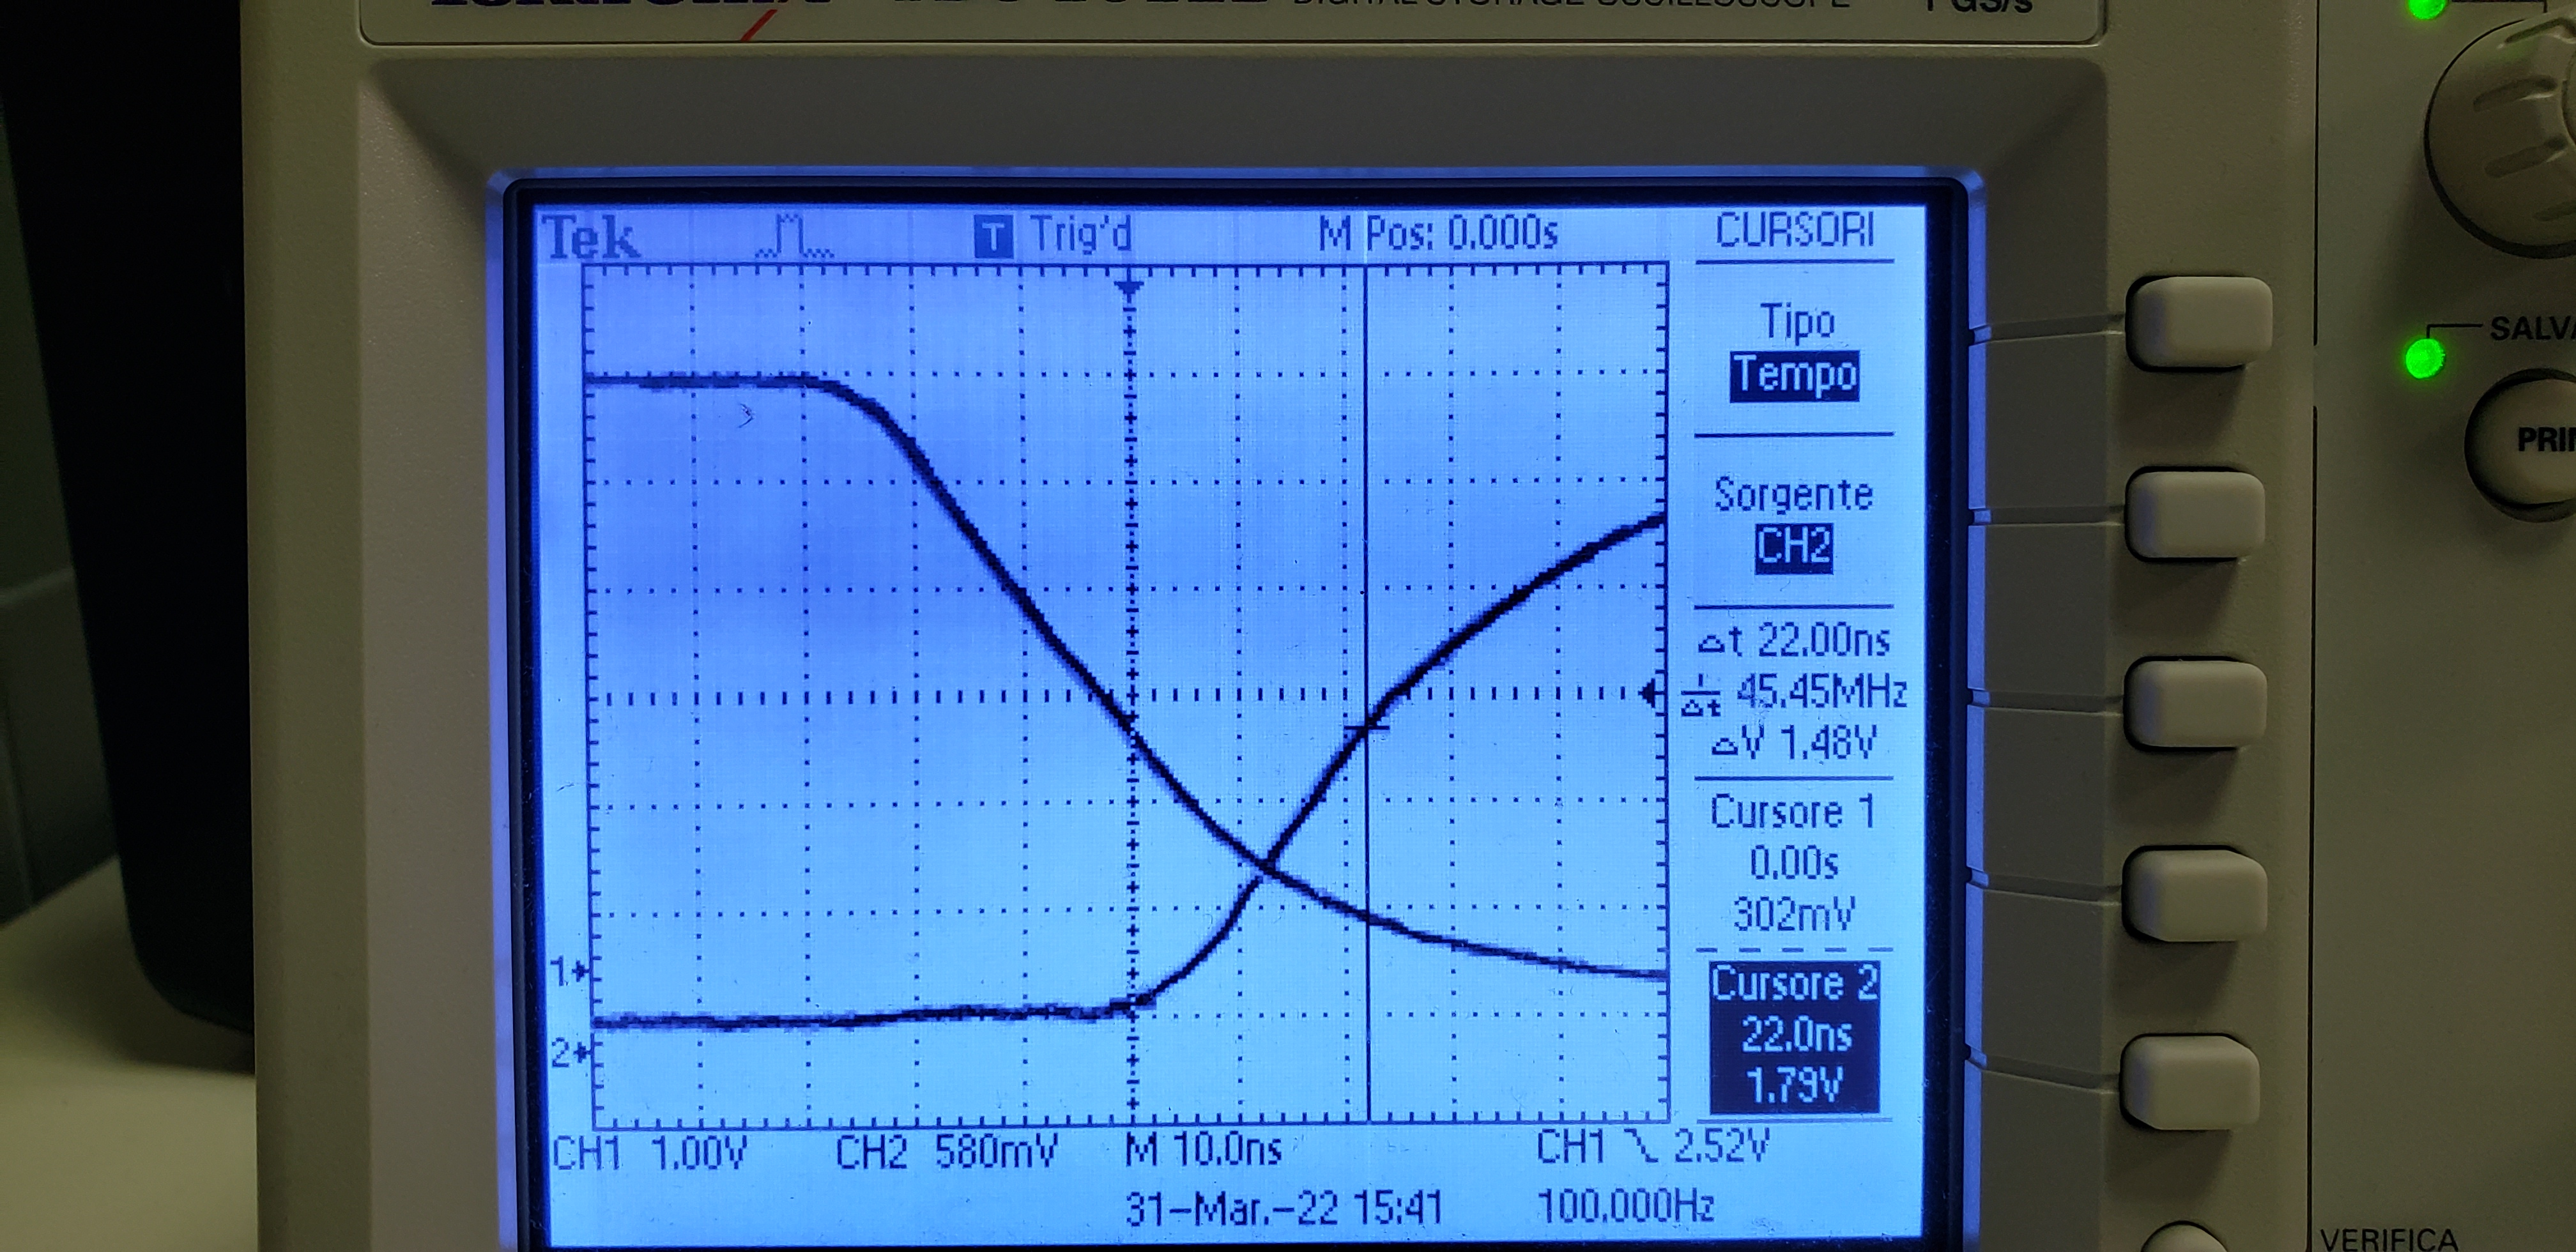
\includegraphics[width=\textwidth]{HL1}
	\caption{Acquisizione tramite oscilloscopio digitale della transizione da
	H a L per il primo integrato}
\end{figure}
\begin{figure}[htbp]
\centering
	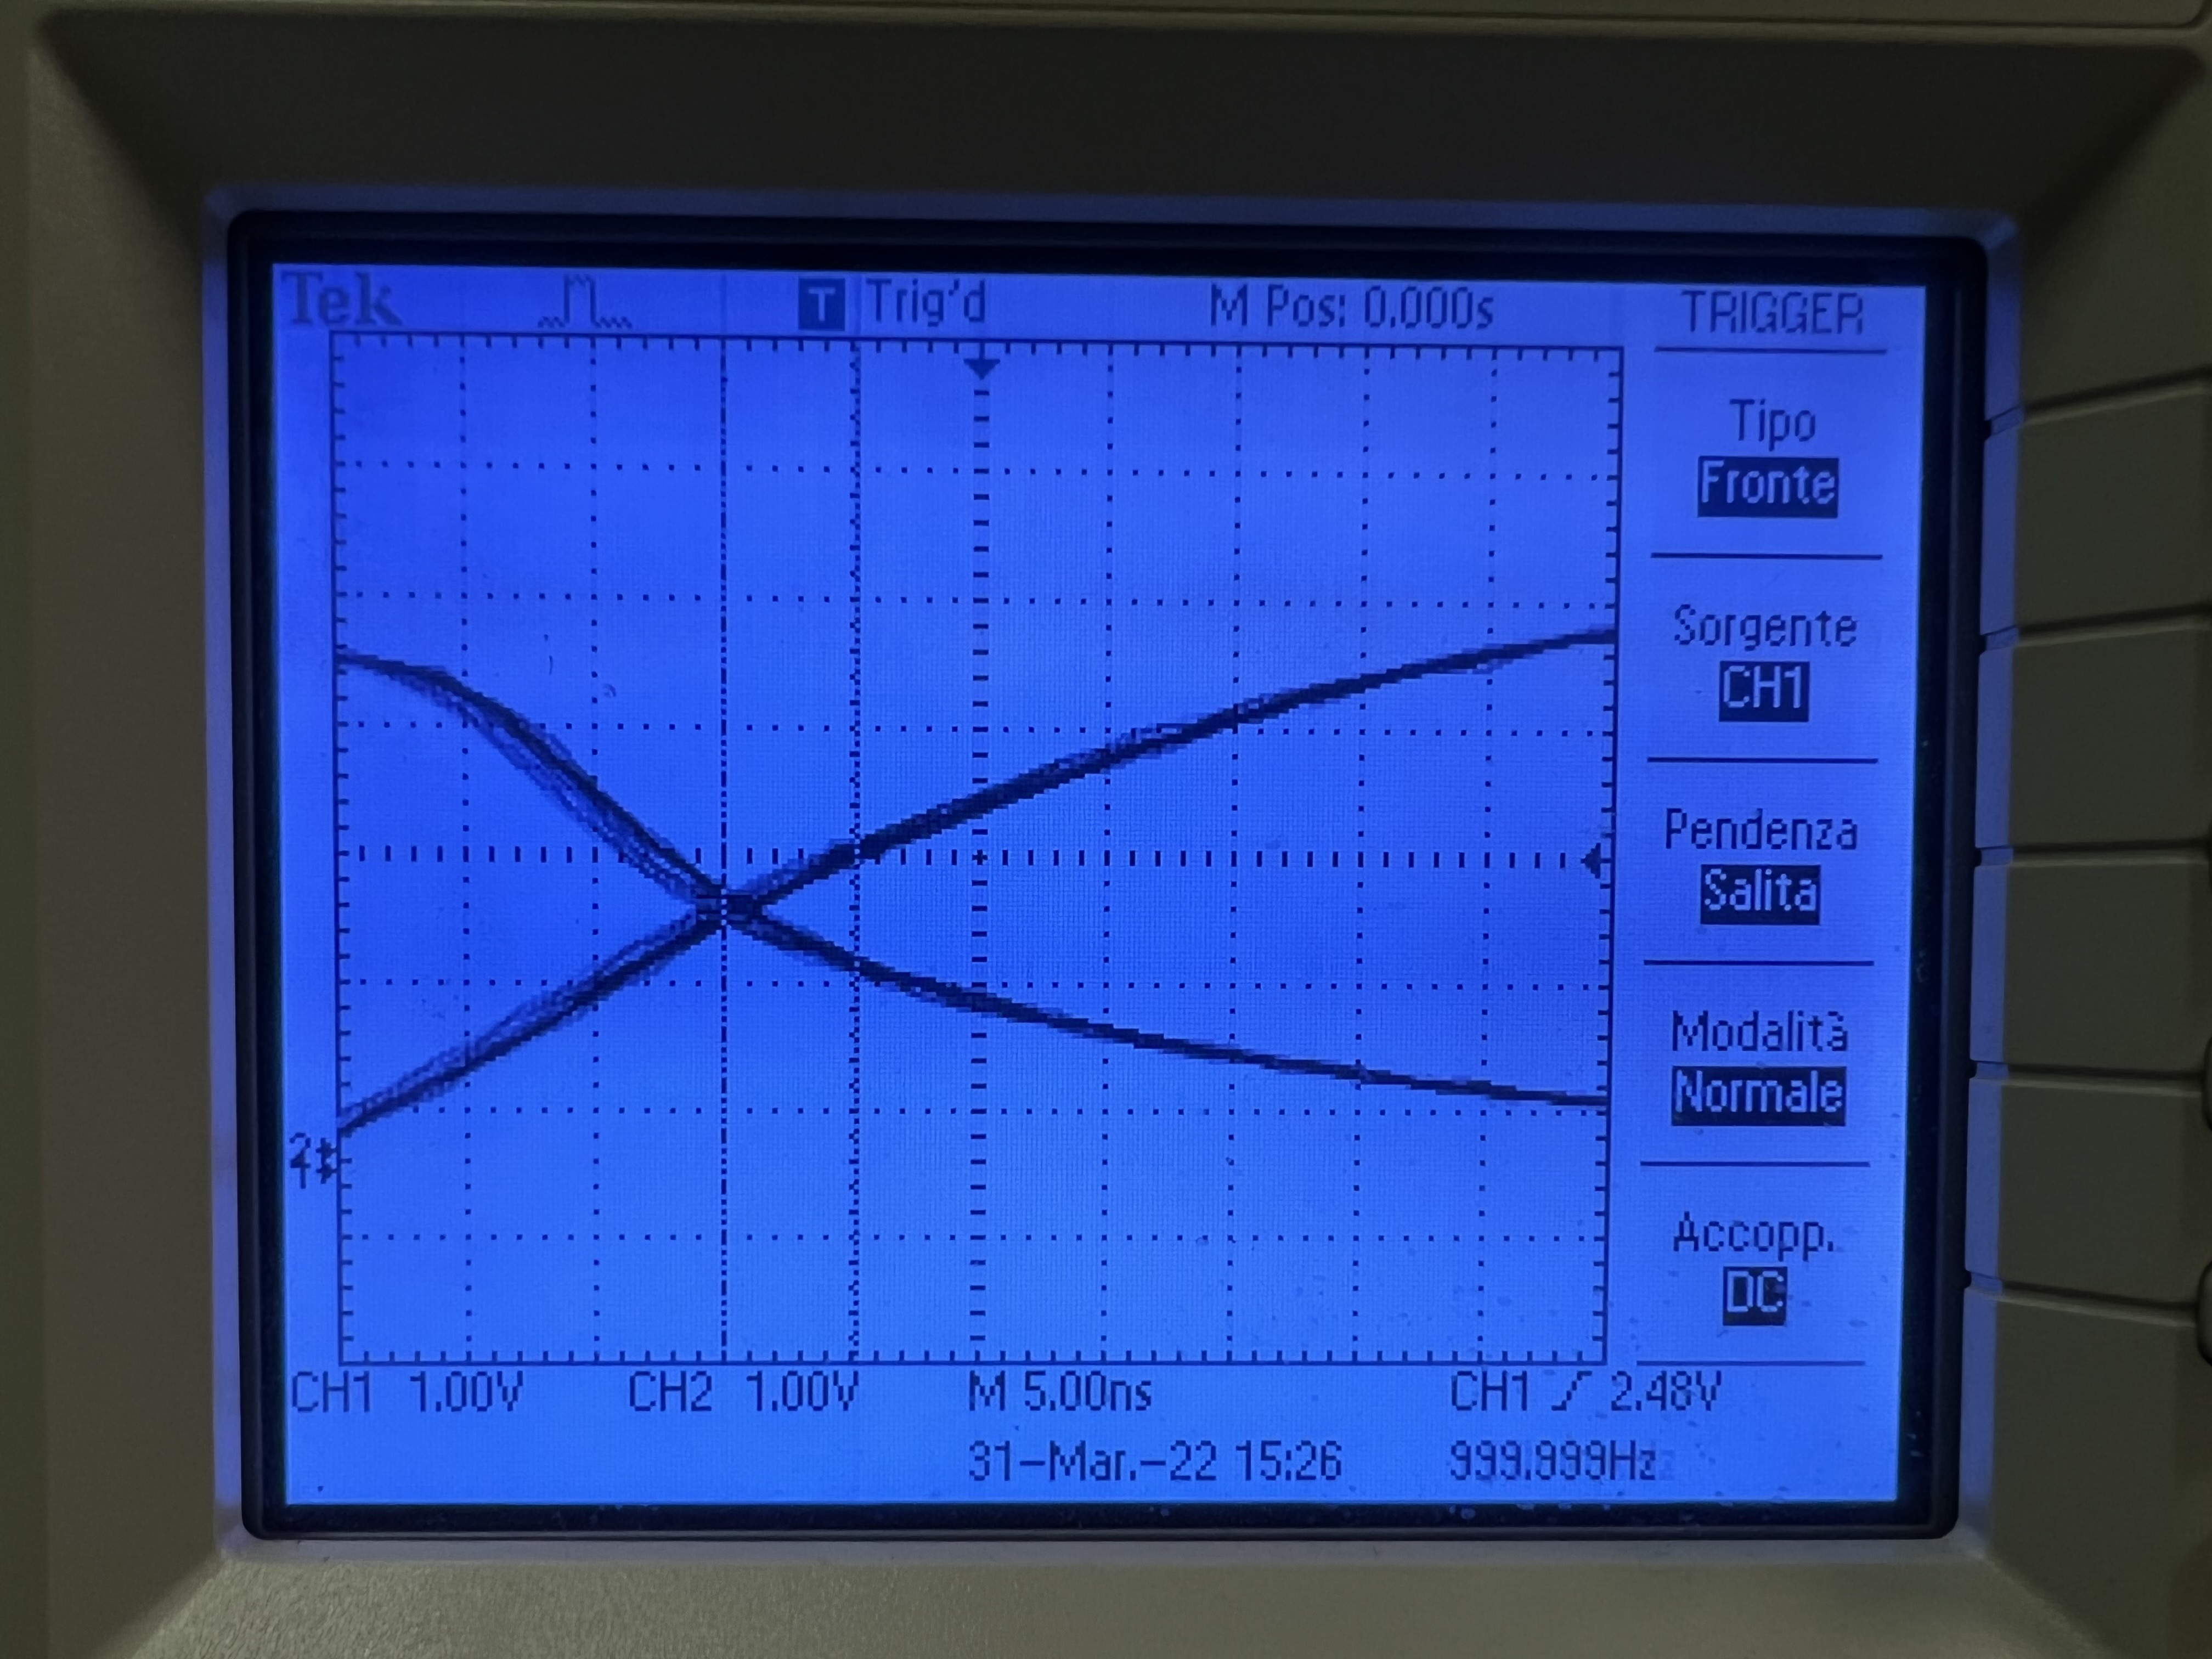
\includegraphics[width=\textwidth]{HL2}
	\caption{Acquisizione tramite oscilloscopio digitale della transizione da
	H a L per il secondo integrato}
\end{figure}

Dalla misura fatta con i cursori sull'oscilloscopio si ricava
\begin{multicols}{2}
    \centering
    $t_{PLH}=$ 5.2 $\pm$ 0.2 \si{n\s} \\
    $t_{PHL}=$ 25.0 $\pm$0.2 \si{n\s}
    
    $t_{PLH}=$ 7.0 $\pm$0.2 \si{n\s} \\
    $t_{PHL}=$ 22.0 $\pm$0.2 \si{n\s}
\end{multicols}

\subsection{Confronto con i valori attesi}
%TODO Scrivere in maniera sensata
Dobbiamo però constatare la presenza di capacità parassite presenti nelle basette e circuito, infatti aumentando la scala dei tempi ci rendiamo conto che tutti i grafici prodotti dall'oscilloscopio rispecchiano qualitativamente il grafico della carica e scarica del condensatore (figura \cref{fig: carica}); per questo motivo si sono ottenuti in alcuni casi dei tempi di propagazione poco più alti delle aspettative, per cui non abbiamo ragione di credere che le nostre misure non siano compatibili con le aspettative.
\begin{figure}[htbp]
\centering
	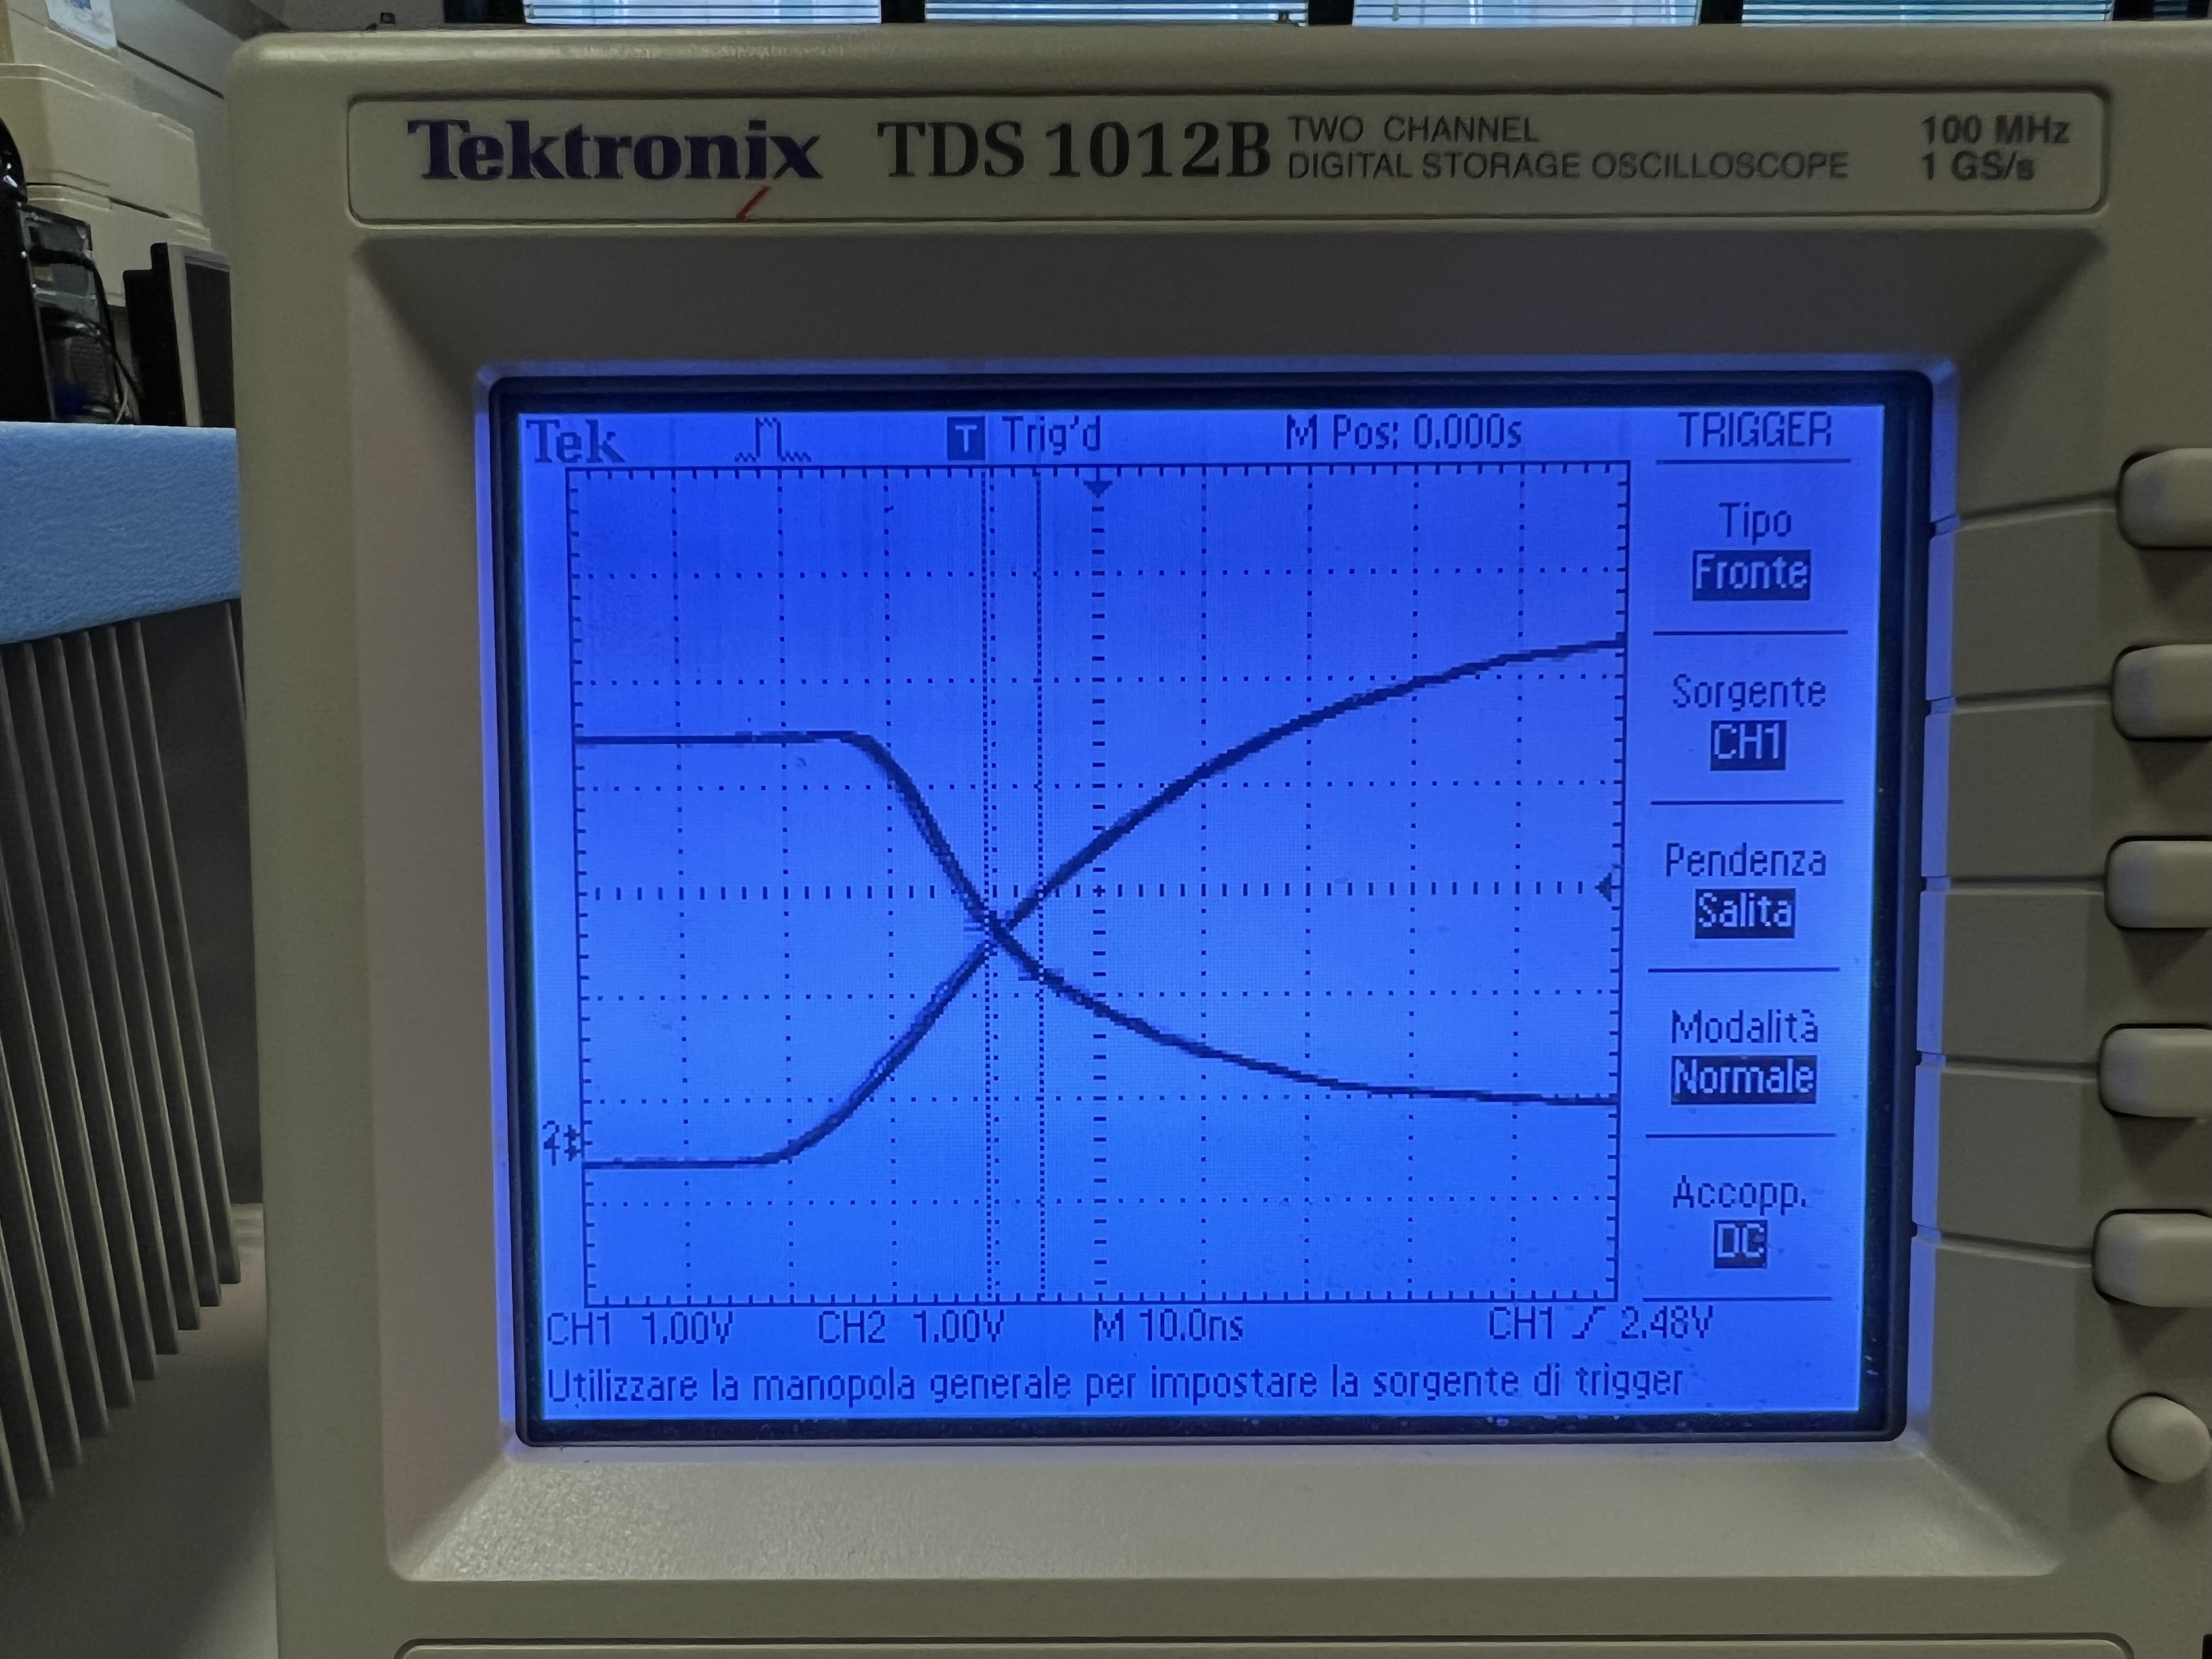
\includegraphics[width=\textwidth]{carica}
	\label{fig: carica}
	\caption{Acquisizione con oscilloscopio digitale con un fondo scala dei tempi più grande, in modo da osservare qualitativamente come la propagazione del segnale assomigli molto al grafico della tensione ai capi di un condensatore durante il ciclo di carica/scarica}
\end{figure}
Possiamo quindi concludere che le misure sono in linea con quanto dichiarato nel datasheet.

\setcounter{section}{3}
%=======================
\section*{Parte B: Circuiti logici elementari con sole porte NAND}
La caratteristica più fondamentale delle porte NAND è la loro universalità,
infatti è possibile realizzare qualsiasi tipo di circuito logico tramite
combinazione di sole porte NAND (o NOR). In questa parte intendiamo costruire
e verificare il funzionamento di circuiti equivalenti a porte OR, XOR e
multiplexer a partire da soli chip NAND SN74LS00.

\begin{figure}[htbp]
\centering
    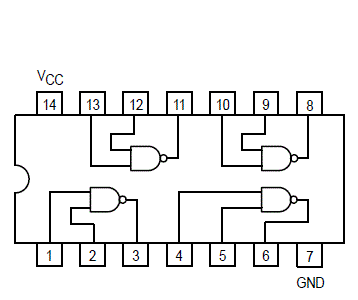
\includegraphics[width=\textwidth]{NAND}
    \caption{Schema circuitale del circuito integrato SN74LS00}
    \label{fig: NAND}
\end{figure}

\section{Tabella di verità}
\subsection{Verifica statica della tabella di verità NAND}
%TODO Non so se vogliamo almeno dire che lo abbiamo fatto senza mettere
% immagini

\subsection{Verifica del funzionamento dinamica con Logic Analyzer}
Definiamo dentro lo strumento Patterns (generator) di WaveForms 2 segnali
di clock rispettivamente a 100 Hz (in uscita dalla porta DIO0 e in ingresso
al pin 1 dell'integrato) e l'altro a 200 Hz (in uscita dalla porta DIO1 e in
entrata nel pin 2) per esplorare tutte le possibili coppie di valori in
ingresso alla porta NAND.

Dunque abbiamo usato lo strumento Logic (Analyzer) per acquisire l'andamento
nel tempo dei segnali presenti nei pin della porta logica utilizzata
(1,2 e 3).
%TODO Non è chiaro che sia questa operazione logica utilizzata (1, 2, 3)

\begin{figure}[htbp]
\centering
	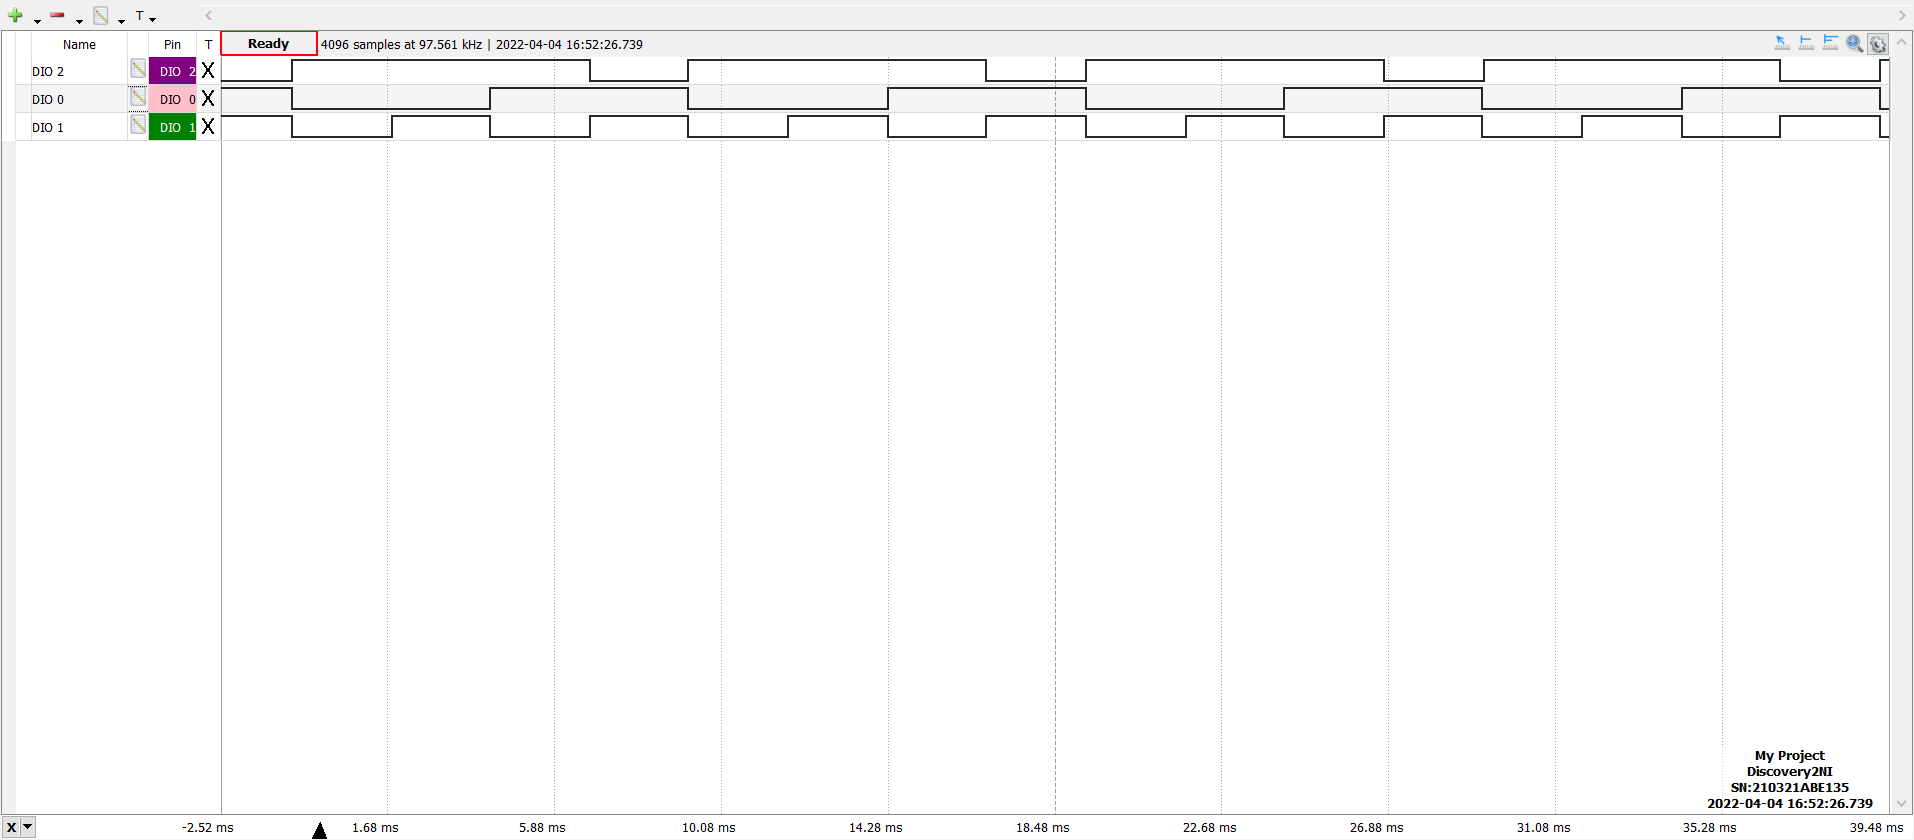
\includegraphics[scale=0.4]{nand_time}
	\caption{Acquisizione di Logic di una porta nand guidata da due segnali da
	DIO0 (100 Hz) e DIO1 (200 Hz); in uscita viene letto da DIO2}
	\label{nand_time}
\end{figure}
Il circuito risulta essere funzionante e l'output risulta essere L se e solo
se i pin 1 e 2 valgono entrambi H, proprio come da aspettative.

\section{Costruzione di circuiti con porte NAND}
\subsection{Porta OR}
Come primo circuito costruiamo una porta OR: detti \textit{A} e \textit{B}
gli ingressi e \textit{Y} l'uscita, nella notazione dell'algebra booleana si ha
\[
    Y = A + B
\]
Sfruttando la legge di De Morgan si ottiene
\[
    Y = A + B = \overline{\overline{A}\cdot\overline{B}}
\]
che descrive la relazione OR in termini del NAND.\\
Nota la relazione per ottenere un NOT utilizzando porte NAND, riportiamo lo schema del circuito
\begin{figure}[htbp]
    \centering
    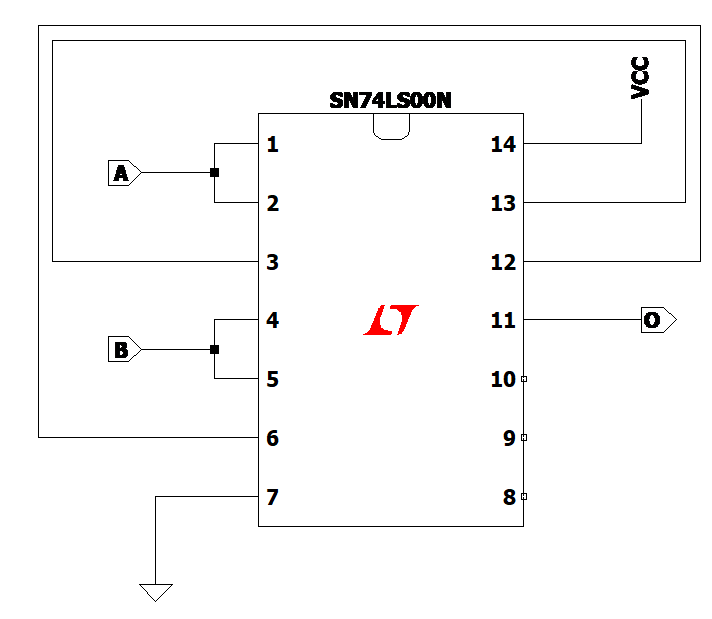
\includegraphics[width=0.45\textwidth]{NAND_OR}
    \caption{\label{fig: OR} Schema circuitale utilizzato per costruire un OR GATE: A e B sono i segnali di input, mentre O è l'output}
\end{figure}

Utilizzando le funzioni pattern e logic abbiamo inviato tramite i pin DIO0 e DIO1 2 segnali di clock di frequenza 50 e 100 Hz e abbiamo utilizzato la porta DIO2 per verificare l'output del circuito
\begin{figure}[htbp]
    \centering
    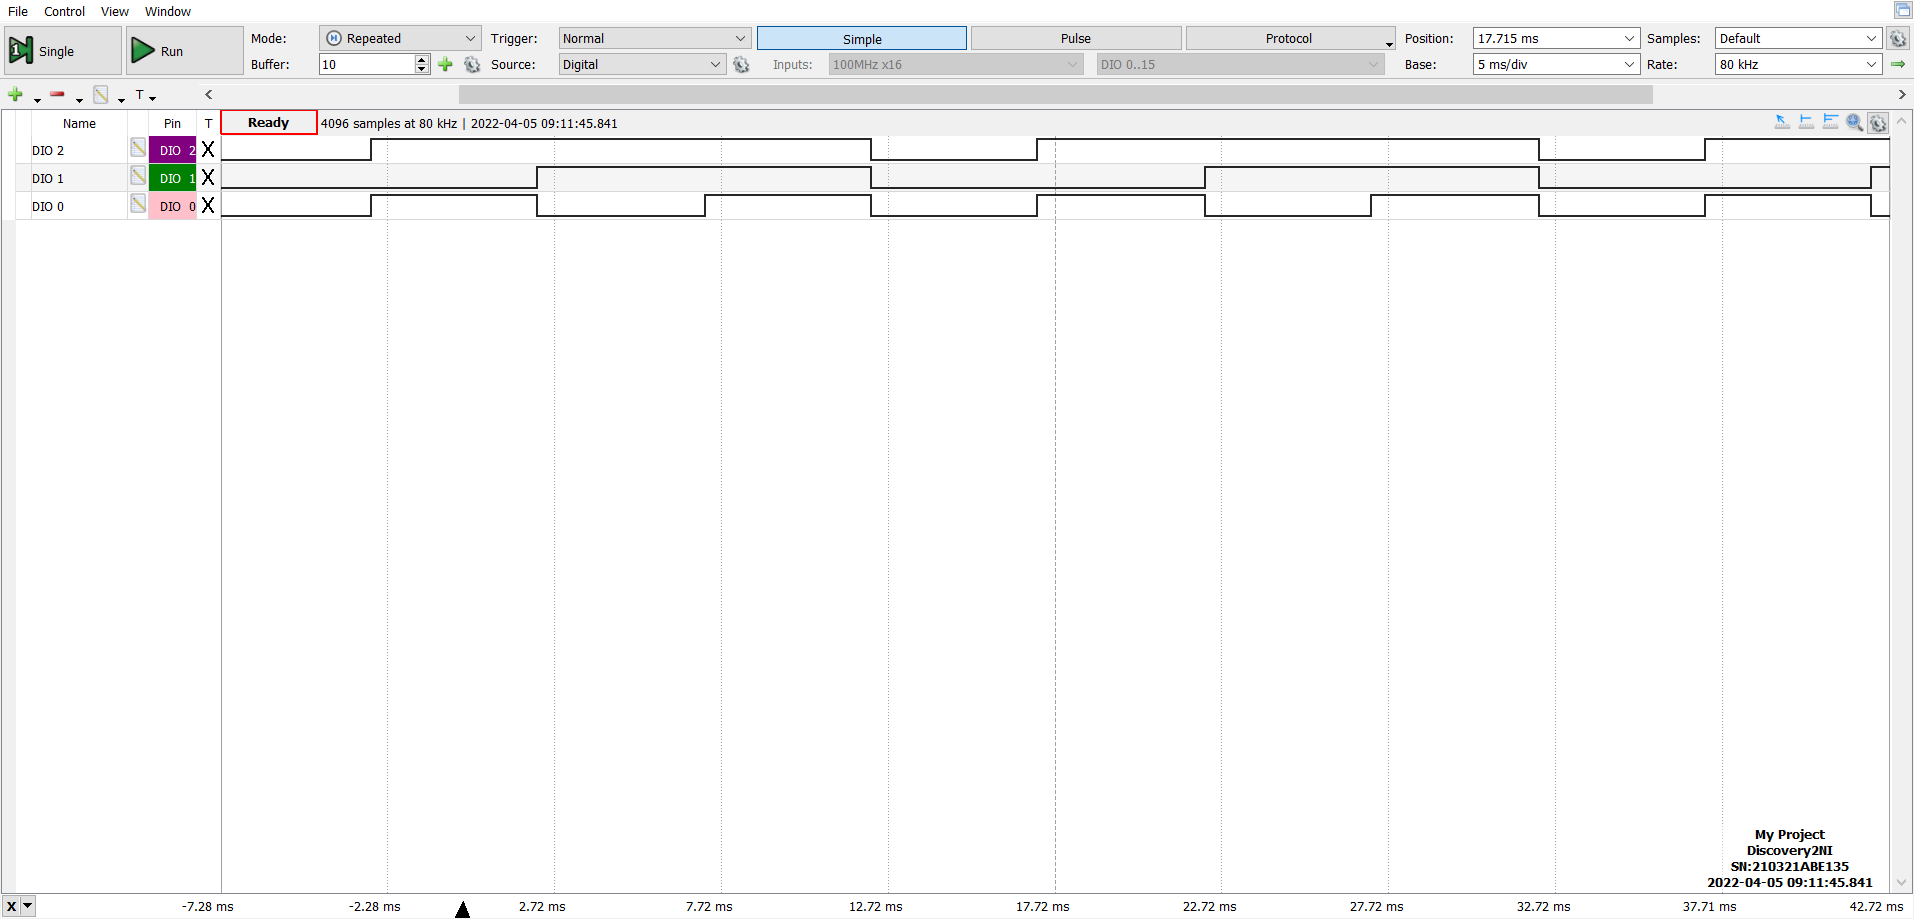
\includegraphics[width=\textwidth]{or_time}
    \caption{Acquisizione Logic per il circuito OR costruito tramite NAND: DIO0 e DIO1 sono i segnali in input, DIO2 è l'output}
\end{figure}
Si vede quindi che il circuito ha il funzionamento aspettato con l'output L se e solo se i due input sono entrambi L.

\subsection{Circuito selettore a due vie (multiplexer)}
Realizziamo un circuito che permetta di assegnare all'uscita il valore di uno dei due ingressi a singolo bit tramite il valore di un terzo ingresso.
Indichiamo con \textit{A}, \textit{B} e \textit{C} gli ingressi e con \textit{Y} l'uscita; 
    \[
    \begin{cases}
    C=0 \implies Y=A\\
    C=1 \implies Y=B
    \end{cases}
    \]
il funzionamento del nostro circuito può essere descritto dalla tabella di Karnaugh riportata sotto\\
\begin{table}
    \centering
    \begin{tabular}{c||c|c|c|c}
        \backslashbox{C}{AB} & 00 & 01 & 11 & 10\\
        \hline
        \hline
        0 & 0 & 0 & 1 & 1\\
        \hline
        1 & 0 & 1 & 1 & 0\\
    \end{tabular}
\end{table}

da cui si ricava facilmente la seguente relazione per il circuito
\[
Y=A\cdot\overline{C}+B\cdot C
\]
e, sempre sfruttando De Morgan, si ha
\[
Y=A\cdot\overline{C}+B\cdot C=\overline{(\overline{A\cdot\overline{C}})\cdot(\overline{B\cdot C})}
\]
Riportiamo sotto lo schema del circuito
\begin{figure}[htbp]
    \centering
    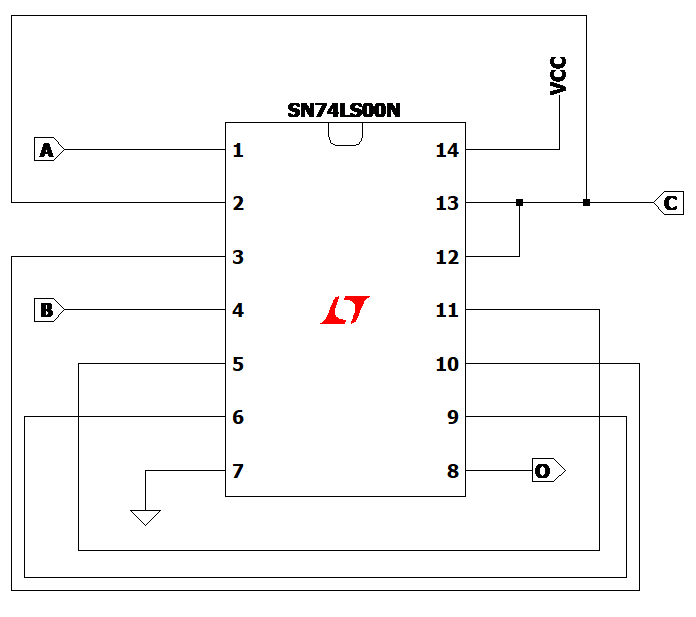
\includegraphics[width=0.6\textwidth]{NAND_MP.png}
    \caption{Schema circuitale per costruire un multiplexer a 2 input, controllato dal valore logico C}
    \label{circuito2}
\end{figure}

Per dimostrare il corretto funzionamento del circuito riportiamo le acquisizioni di Pattern, in cui è possibile comprendere come sono stati impostati gli ingressi, e Logic, da cui si può verificare il corretto funzionamento del circuito.
Abbiamo inviato al circuito tramite la funzione pattern un segnale di clock a 100 Hz a B, uno a 50 Hz a A e infine uno a 25 Hz a C.
\begin{figure}[htbp]
    \centering
    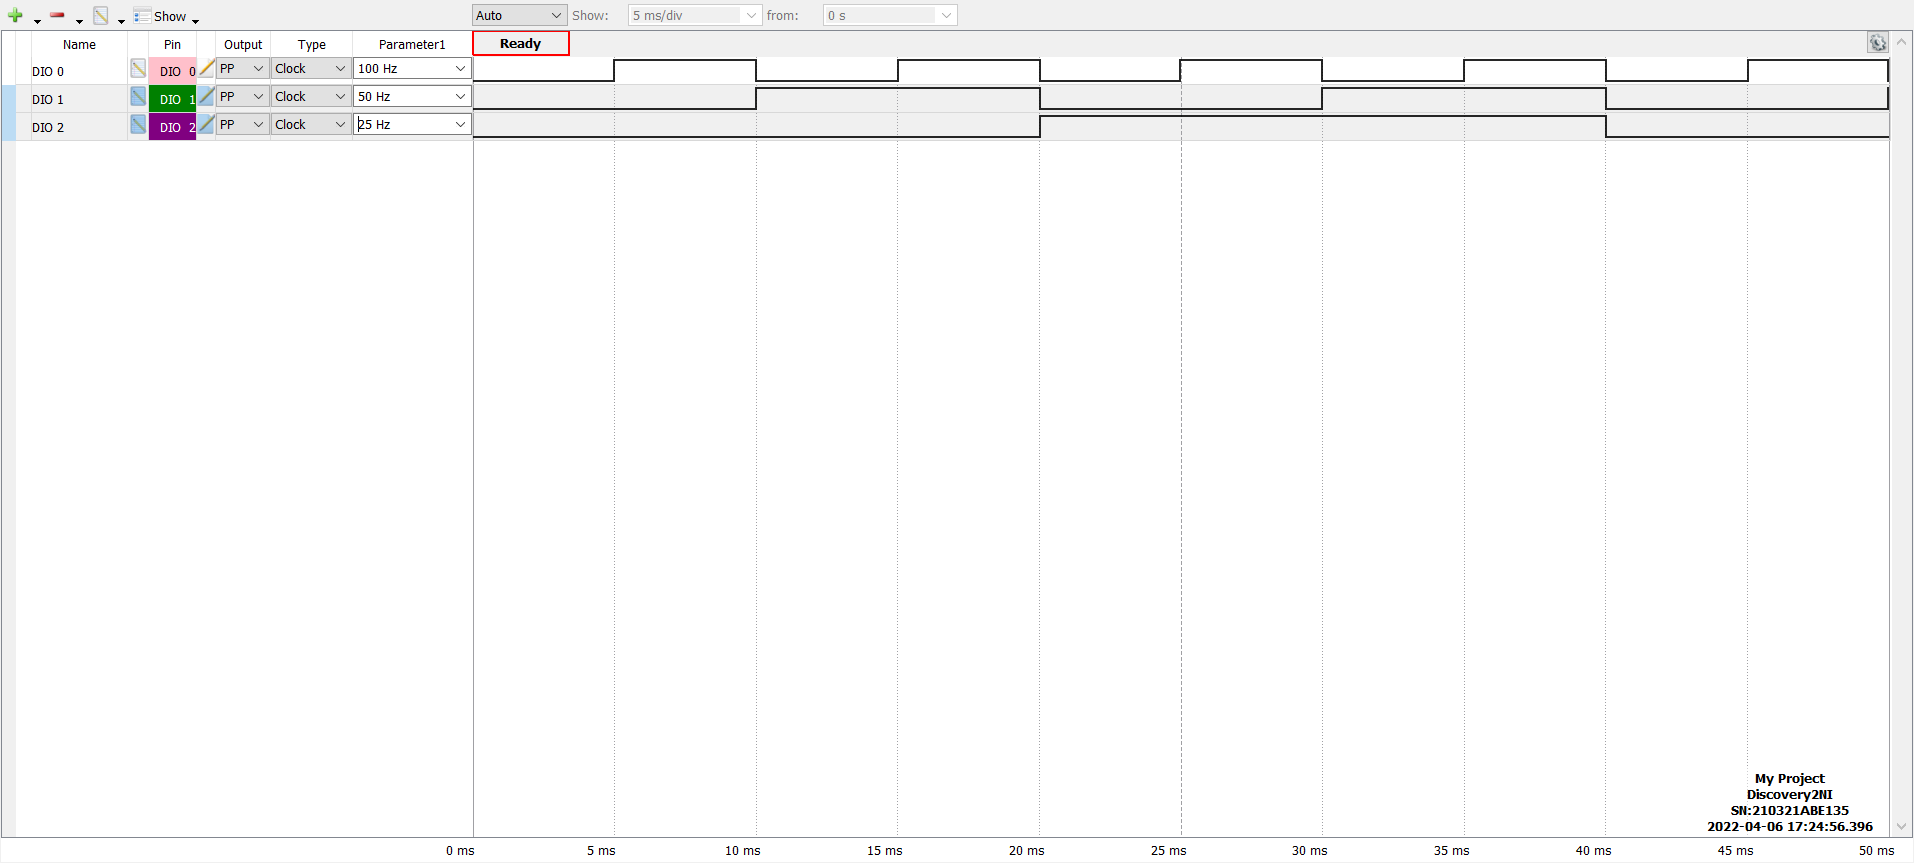
\includegraphics[width=0.8\textwidth]{pat2.png}
    \caption{Logic: DIO 0 $\equiv$ B, DIO 1 $\equiv$ A, DIO 2 $\equiv$ C}
    \label{logic2}
\end{figure}
\begin{figure}[htbp]
    \centering
    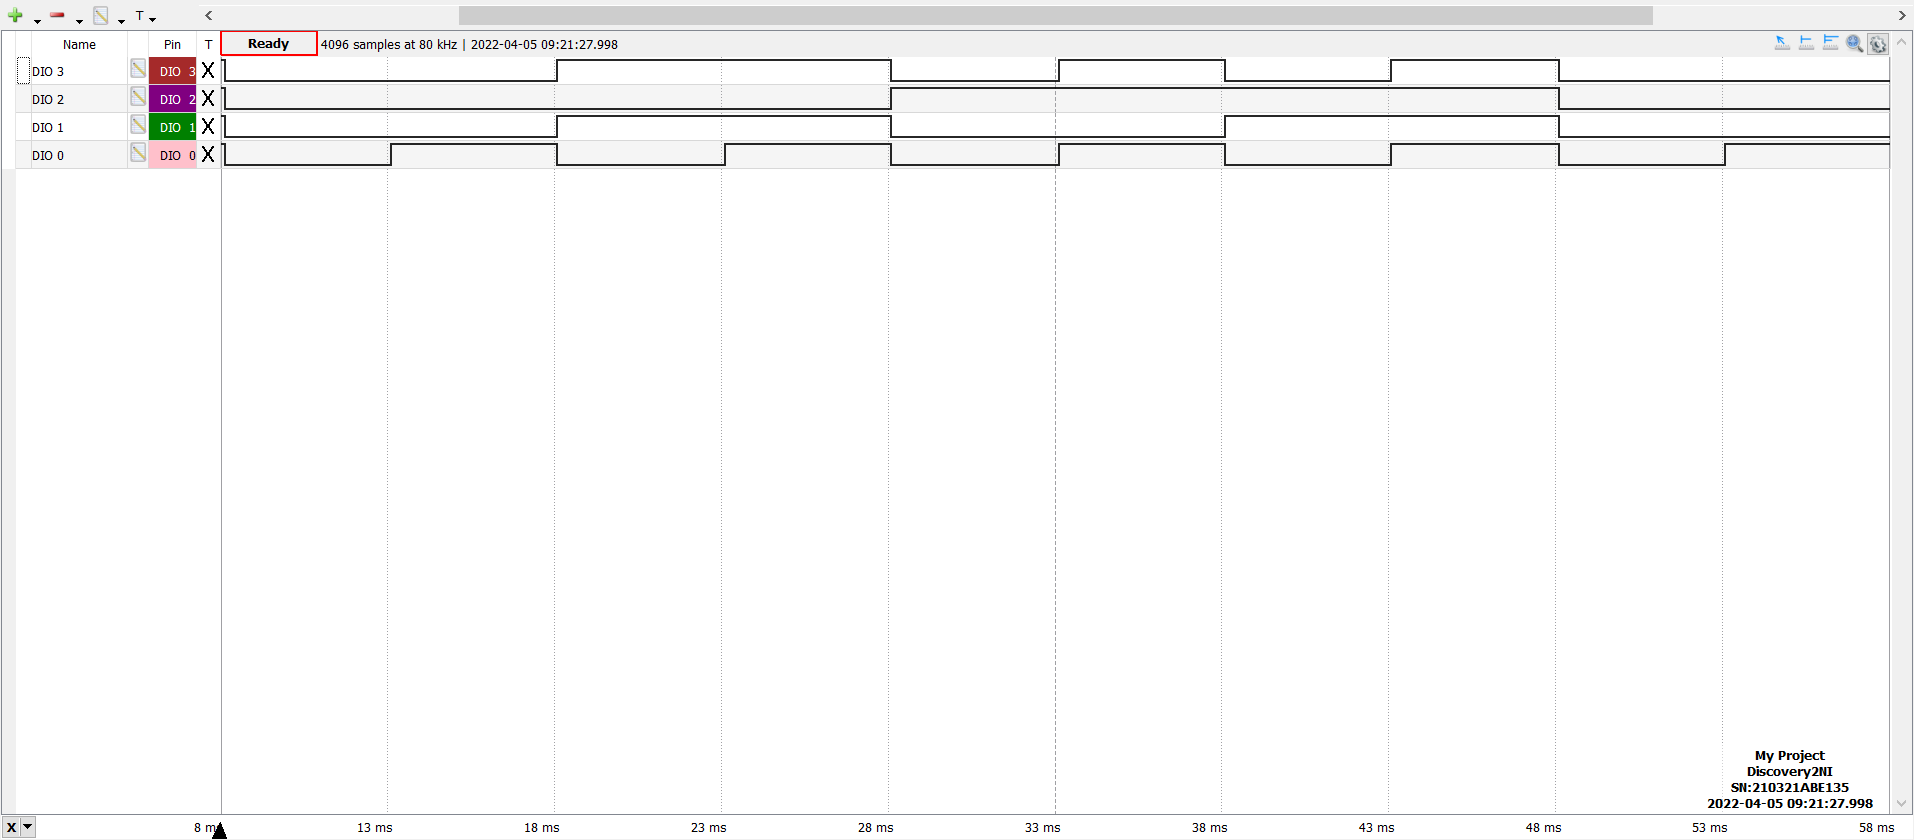
\includegraphics[width=0.8\textwidth]{Multiplex.png}
    \caption{Logic: DIO 0 $\equiv$ B, DIO 1 $\equiv$ A, DIO 2 $\equiv$ C, DIO 3 $\equiv$ Y}
    \label{logic2}
\end{figure}
Si ricava quindi che il circuito funziona come da aspettative, restituendo il segnale di A nel caso in cui C=0 e il segnale B quando C=1.


\subsection{Porta XOR}
Un circuito \texttt{XOR} si può realizzare con 4 porte \texttt{NAND} partendo
dalla sua equazione caratteristica e manipolandola con le leggi di De Morgan:
\begin{align*}
  A \oplus B &= (A \cdot \overline{B}) + (\overline{A} \cdot B)
             =  (A \cdot \overline{A} + A \cdot \overline{B}) + (B \cdot \overline{B} + \overline{A} \cdot B) \\
             &= A \cdot (\overline{A} + \overline{B}) + B \cdot (\overline{B} + \overline{A})
             = A \cdot \overline{(A \cdot B)} + B \cdot \overline{(B \cdot A)} \\
\end{align*}
\begin{figure}[htbp]
    \centering
    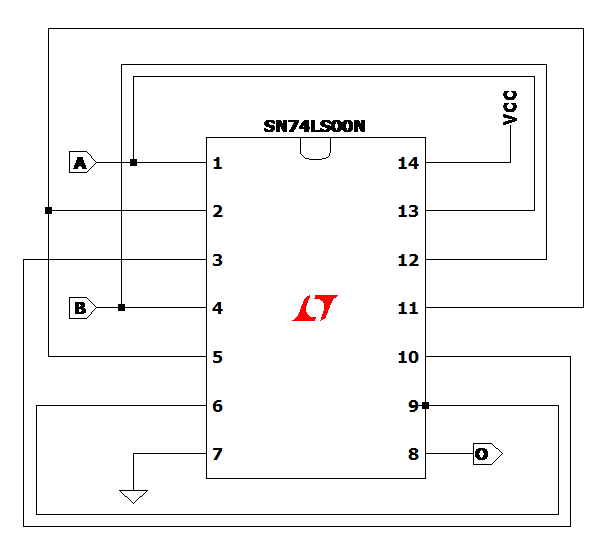
\includegraphics[width=0.6\textwidth]{NAND_XOR.png}
    \caption{Schema circuitale utilizzato per costruire uno XOR GATE tramite NAND}
    \label{circuito3}
\end{figure}

\begin{figure}[htbp]
    \centering
    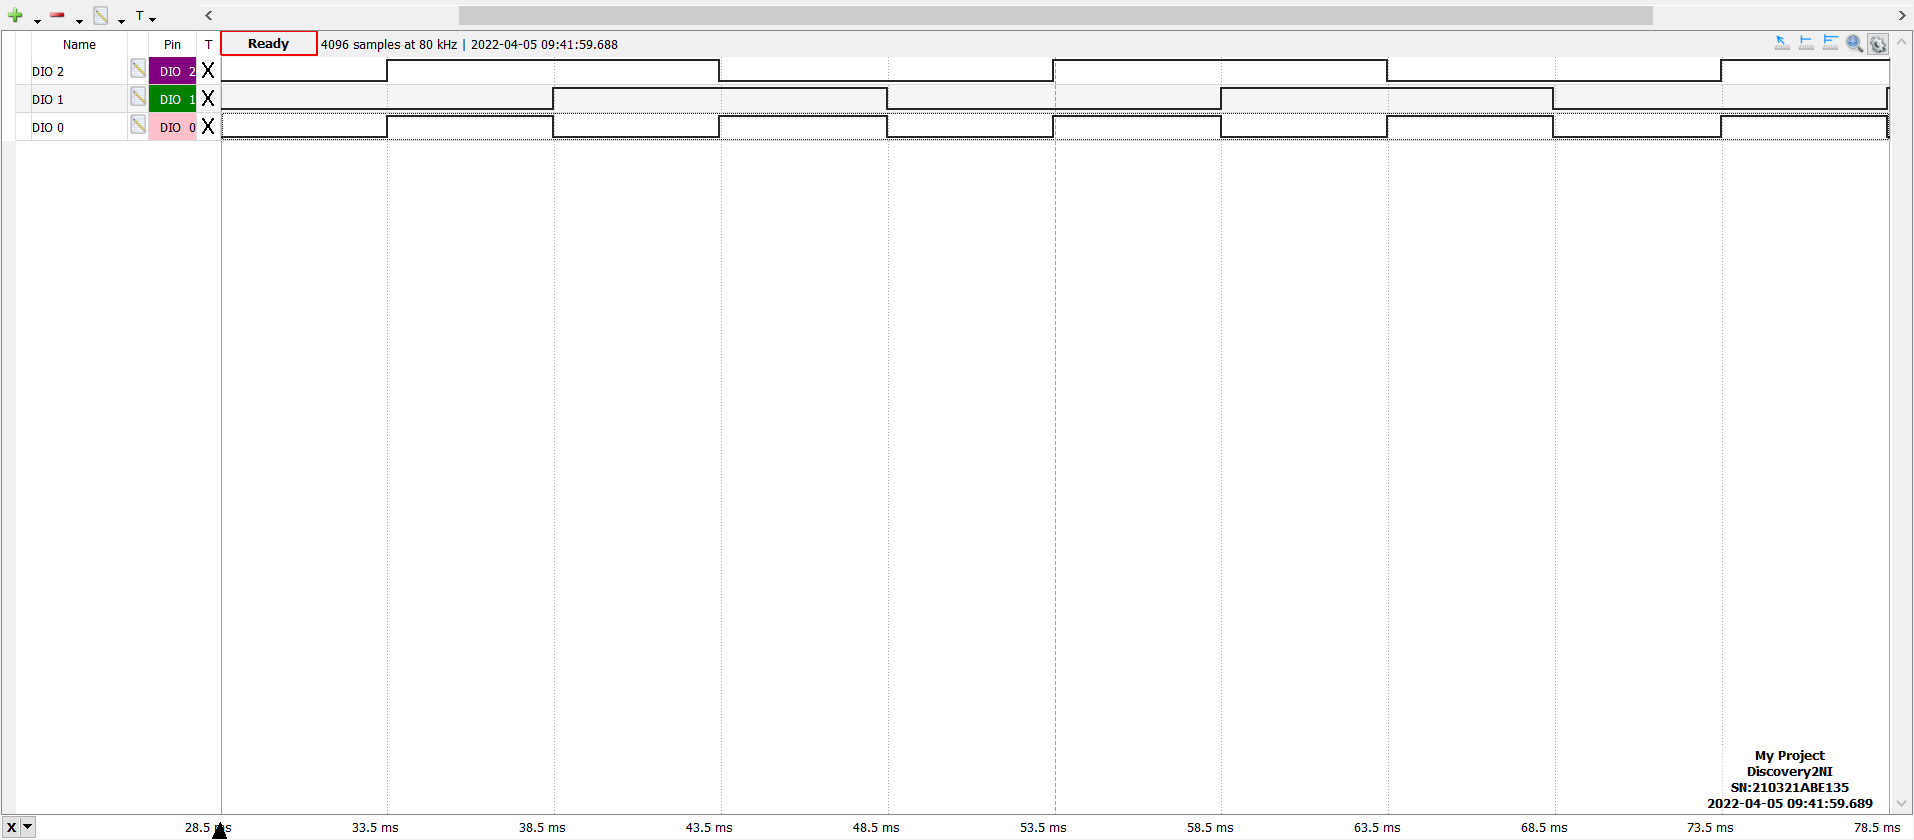
\includegraphics[width=0.8\textwidth]{xor_time.png}
    \caption{Acquisizione Logic della Porta XOR: DIO0 e DIO1 sono i segnali di input, DIO2 è l'uscita dallo XOR}
    \label{pat2}
\end{figure}

Se ne deduce che il circuito ha il funzionamento aspettato e che quindi l'output risulta essere L se e solo se entrambi gli input A e B hanno lo stesso valore.

\setcounter{section}{5}
%=======================
\section*{Parte C: Circuiti logici complessi a più chip}
\section{Convertitore Gray-Binario}
\begin{minipage}{0.7\textwidth}
    Come ultima cosa vogliamo realizzare un circuito in grado di convertire un valore a 4 bit dalla codifica Gray in Binario utilizzando un solo integrato di tipo SN74LS86 a porte XOR, descritto nella figura a lato.\\
    Un convertitore Gray-Binario può essere schematizzato come in Figura (\ref{gb}): il nostro obiettivo è quello di verificare che tale circuito si comporti come atteso.
\end{minipage}
\begin{minipage}{0.3\textwidth}
    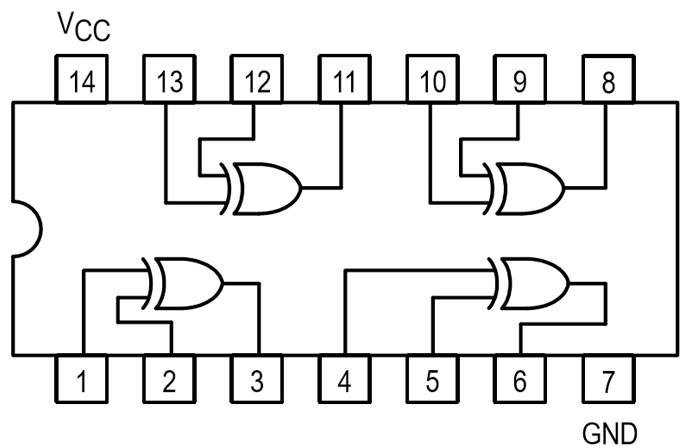
\includegraphics[width=\textwidth]{XOR.png}
\end{minipage}
\newline
\begin{minipage}{0.5\textwidth}
    \centering
    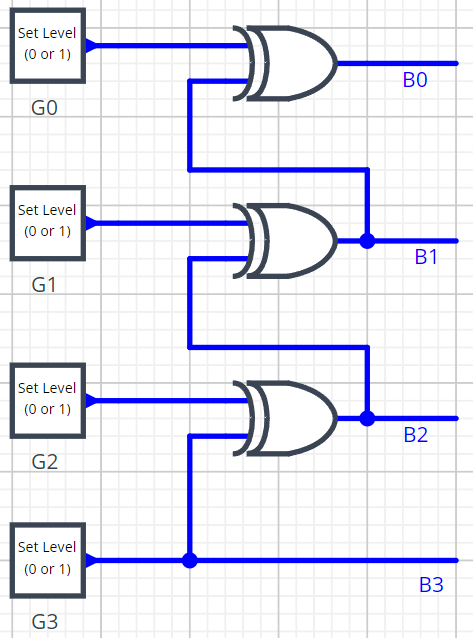
\includegraphics[width=0.8\textwidth]{gb.png}
    \captionof{figure}{Schema convertitore Gray-Binario}
    \label{gb}
\end{minipage}

\begin{table}[htbp]
    \centering
    \begin{tabular}{c||c}
        Codice binario & Codice Gray \\
        \hline
        \hline
        0000 & 0000\\
        0001 & 0001\\
        0010 & 0011\\
        0011 & 0010\\
        0100 & 0110\\
        0101 & 0111\\
        0110 & 0101\\
        0111 & 0100\\
        1000 & 1100\\
        1001 & 1101\\
        1010 & 1111\\
        1011 & 1110\\
        1100 & 1010\\
        1101 & 1011\\
        1110 & 1001\\
        1111 & 1000\\
        \end{tabular}
    \caption{Conteggio a 4 bit nei due codici.}
    \label{tab: grbin}
\end{table}

Il codice Gray differisce dal codice binario in quanto si passa da un intero al successivo modificando un solo bit per volta.\\
Calcoliamo l'uscita del circuito per alcuni valori in ingresso:
\begin{table}[htbp]
    \centering
    \[
    \begin{array}{cccc|cccc}
        G_3 & G_2 & G_1 & G_0 & B_3 & B_2 & B_1 & B_0\\
        \hline
        0 & 0 & 0 & 0 & 0 & 0 & 0 & 0\\
        1 & 1 & 1 & 1 & 1 & 0 & 1 & 0\\
        1 & 0 & 0 & 1 & 1 & 1 & 1 & 0\\
        1 & 0 & 0 & 0 & 1 & 1 & 1 & 1\\
    \end{array}
    \]
\end{table}

Confrontando le uscite ottenute con i valori riportati in \cref{tab: grbin} affermiamo che il circuito si comporta correttamente come convertitore Gray-Binario. Come conferma, riportiamo un'acquisizione.\\
\begin{figure}[htbp]
    \centering
    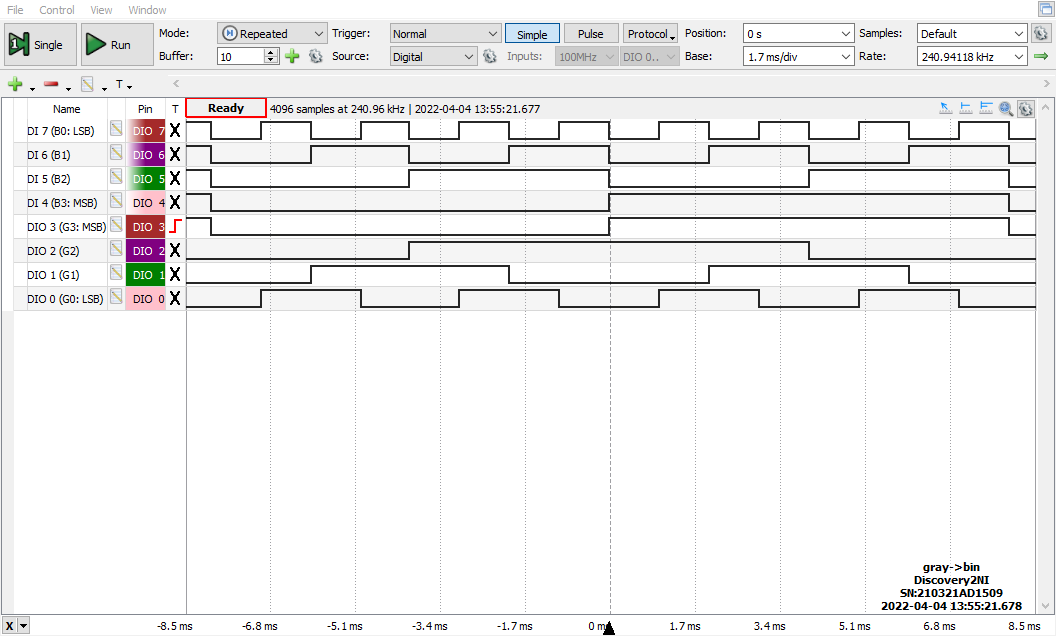
\includegraphics[width=\textwidth]{graybin}
    \caption{Acquisizione di un ciclo completo (frequenza 1 kHz) con Logic
    Analyzer dei segnali in ingresso e in uscita dal convertitore Gray-binario.}
\end{figure}
\begin{figure}[htbp]
    \centering
    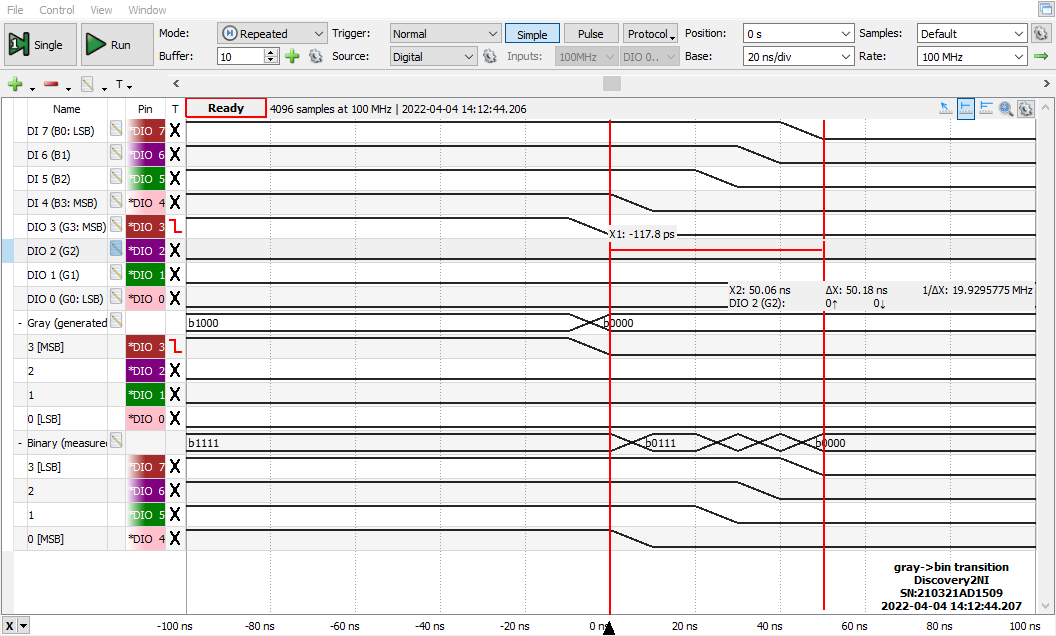
\includegraphics[width=\textwidth]{gray20ns}
    \caption{Acquisizione del Logic Analyzer durante la transizione dal numero $15$ al numero $0$ su scala dei tempi pari a $20$ ns.}
\end{figure}
Per una scala dei tempi molto stretta, si registra che i tempi di propagazione non sono istantanei, distinguendo dei glitch sui canali di uscita. \\ 

\begin{figure}[htbp]
    \centering
    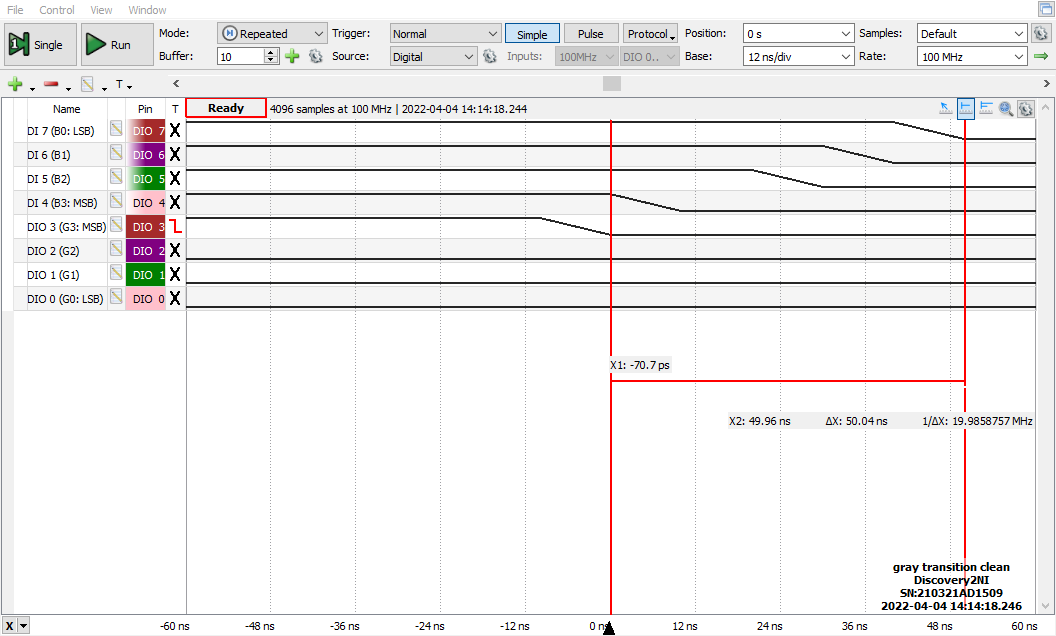
\includegraphics[width=\textwidth]{gray10ns}
    \caption{Transizione dal $15$ allo $0$ su scala temporale pari a $10$ ns.}
\end{figure}
(verificate il funzionamento del circuito utilizzando Pattern per generare un contatore a 4 bit con la codifica opportuna e osservando l’uscita con Logic (come ai punti precedenti);\\
%TODO motivare l’osservazione del punto precedente tenendo conto del tempo di propagazione necessario per i due circuiti;\\

%TODO riportare tutti i grafici necessari a dimostrare il funzionamento del circuito

\section{Sommatore a 2 bit}
Vogliamo costruire un sommatore a due bit utilizzando le dovute porte logiche. Utilizzeremo i chip \texttt{SN74LS08} (quad-AND), \texttt{SN74LS32} (quad-OR), \texttt{SN74LS86} (quad-XOR). Il circuito da montare è riportato in \cref{fig: sommatore}.

\begin{figure}[htbp]
    \centering
    \includegraphics[width=0.6\linewidth]{half.png}
    \caption{Schema circuitale di un half adder}
    \label{fig:halfadder}
\end{figure}

\begin{figure}[htbp]
    \centering
    \includegraphics[width=0.6\linewidth]{full.png}
    \caption{Schema circuitale di un full adder.}
    \label{fig:fulladder}
\end{figure}

\begin{figure}[htbp]
    \centering
    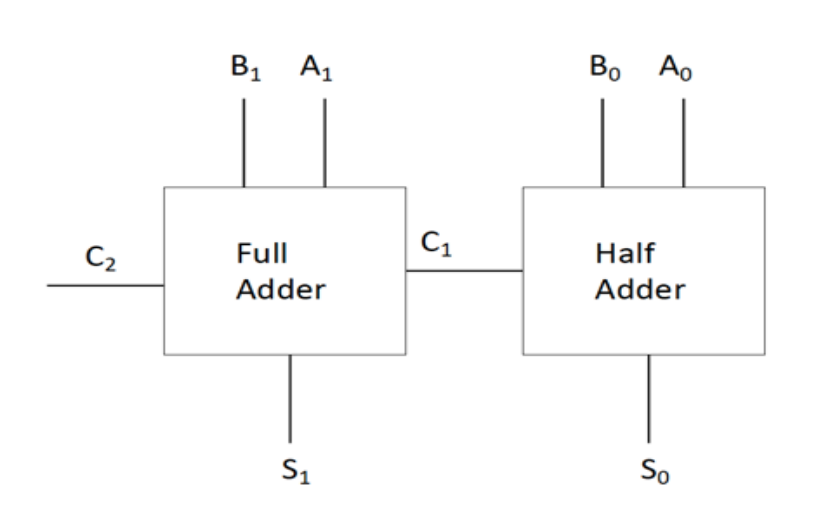
\includegraphics[width=0.6\linewidth]{sum.png}
    \caption{Schema circuitale di un sommatore a 2 bit}
    \label{fig: sommatore}
\end{figure}

Verifichiamo il funzionamento mandando in ingresso tutte le possibili combinazioni di due numeri a due bit. Per fare ciò mandiamo ai 4 ingressi del circuito un segnale che conta in binario. Il risultato è mostrato in \cref{fig: faAD2}.

\begin{figure}[htbp]
    \centering
    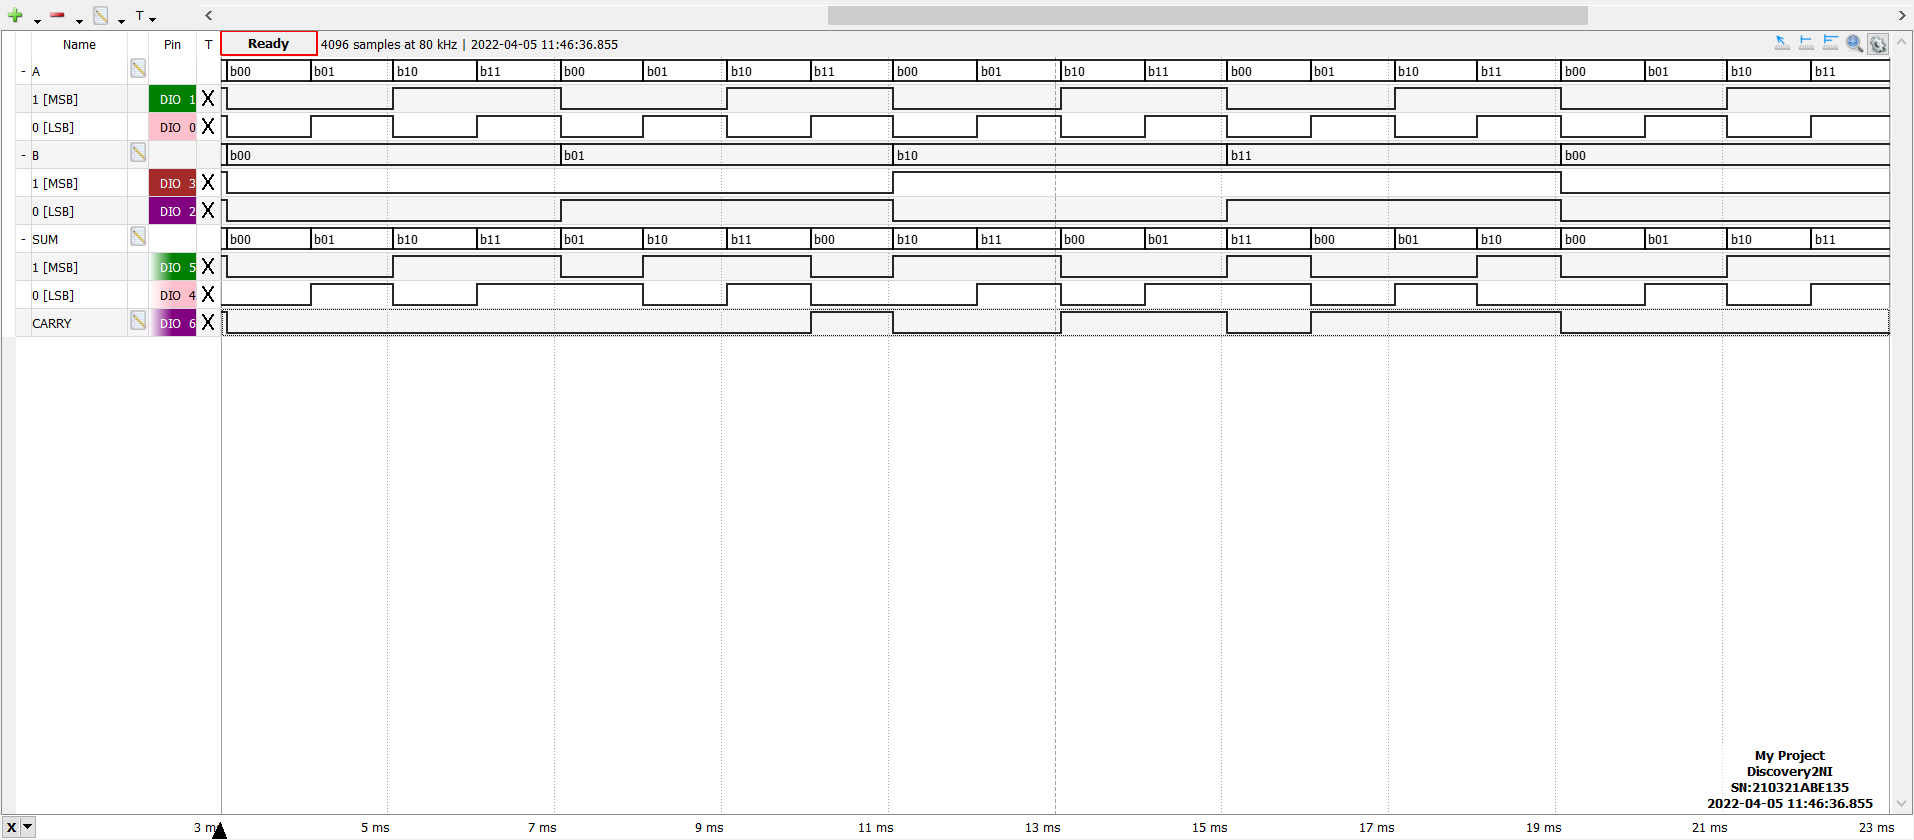
\includegraphics[width=\linewidth]{sum_time.png}
    \caption{Acquisizione Logic per il sommatore a 2 bit: DIO0 e DIO1 rappresentano il numero A; DIO2 e DIO3 rappresentano B; DIO4, DIO5 e DIO6 rappresentano invece rispettivamente il risultato della somma (con DIO4 il LSB) e il bit di overflow}
    \label{fig: faAD2}
\end{figure}

Aggiungiamo al circuito 4 led verdi e un led rosso: questi sono pilotati da 5 nuovi cavi dell'AD2. Per controllare il loro funzionamento aggiungiamo a \emph{Patterns} una tabella delle verità, riportata in \cref{fig: Ver}, che faccia in modo che ad ogni step si illuminino un numero di led pari al valore della somma. Il led rosso verrà usato per controllare l'overflow, ovvero la possibilità che il risultato sia maggiore o uguale a 4.

\begin{figure}[htbp]
    \centering
    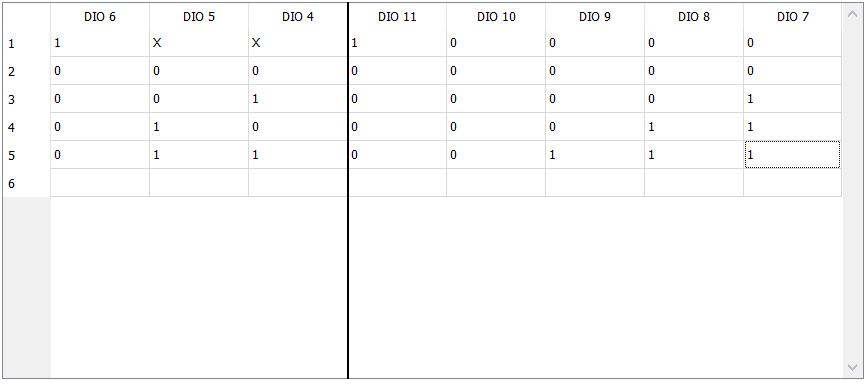
\includegraphics[width=0.8\linewidth]{TAB_LED}
    \caption{Tabella delle verità usata per il controllo dei led.}
    \label{fig: Ver}
\end{figure}

%=======================
\section*{Conclusioni e commenti finali}
Si è riusciti a verificare il corretto comportamento delle porte TTL studiate
caratterizzandone le tensioni, correnti di operazione e tempi caratteristici
di circuiti integrati come il SN7404.
Inoltre, è stato possibile verificare il funzionamento di circuiti logici di
diversa complessità costruiti con porte NAND, XOR, e OR e si è riusciti ad
apprezzare l'effetto dei tempi di propagazione delle porte nella conversione
dalla codifica Gray al binario.

%=======================
\section*{Dichiarazione}
I firmatari di questa relazione dichiarano che il contenuto della relazione \`e
originale, con misure effettuate dai membri del gruppo, e che tutti i firmatari
hanno contribuito alla elaborazione della relazione stessa.

\end{document}
